% Options for packages loaded elsewhere
\PassOptionsToPackage{unicode}{hyperref}
\PassOptionsToPackage{hyphens}{url}
\PassOptionsToPackage{dvipsnames,svgnames,x11names}{xcolor}
%
\documentclass[
  letterpaper,
  DIV=11,
  numbers=noendperiod]{scrartcl}

\usepackage{amsmath,amssymb}
\usepackage{iftex}
\ifPDFTeX
  \usepackage[T1]{fontenc}
  \usepackage[utf8]{inputenc}
  \usepackage{textcomp} % provide euro and other symbols
\else % if luatex or xetex
  \usepackage{unicode-math}
  \defaultfontfeatures{Scale=MatchLowercase}
  \defaultfontfeatures[\rmfamily]{Ligatures=TeX,Scale=1}
\fi
\usepackage{lmodern}
\ifPDFTeX\else  
    % xetex/luatex font selection
\fi
% Use upquote if available, for straight quotes in verbatim environments
\IfFileExists{upquote.sty}{\usepackage{upquote}}{}
\IfFileExists{microtype.sty}{% use microtype if available
  \usepackage[]{microtype}
  \UseMicrotypeSet[protrusion]{basicmath} % disable protrusion for tt fonts
}{}
\makeatletter
\@ifundefined{KOMAClassName}{% if non-KOMA class
  \IfFileExists{parskip.sty}{%
    \usepackage{parskip}
  }{% else
    \setlength{\parindent}{0pt}
    \setlength{\parskip}{6pt plus 2pt minus 1pt}}
}{% if KOMA class
  \KOMAoptions{parskip=half}}
\makeatother
\usepackage{xcolor}
\setlength{\emergencystretch}{3em} % prevent overfull lines
\setcounter{secnumdepth}{5}
% Make \paragraph and \subparagraph free-standing
\makeatletter
\ifx\paragraph\undefined\else
  \let\oldparagraph\paragraph
  \renewcommand{\paragraph}{
    \@ifstar
      \xxxParagraphStar
      \xxxParagraphNoStar
  }
  \newcommand{\xxxParagraphStar}[1]{\oldparagraph*{#1}\mbox{}}
  \newcommand{\xxxParagraphNoStar}[1]{\oldparagraph{#1}\mbox{}}
\fi
\ifx\subparagraph\undefined\else
  \let\oldsubparagraph\subparagraph
  \renewcommand{\subparagraph}{
    \@ifstar
      \xxxSubParagraphStar
      \xxxSubParagraphNoStar
  }
  \newcommand{\xxxSubParagraphStar}[1]{\oldsubparagraph*{#1}\mbox{}}
  \newcommand{\xxxSubParagraphNoStar}[1]{\oldsubparagraph{#1}\mbox{}}
\fi
\makeatother


\providecommand{\tightlist}{%
  \setlength{\itemsep}{0pt}\setlength{\parskip}{0pt}}\usepackage{longtable,booktabs,array}
\usepackage{calc} % for calculating minipage widths
% Correct order of tables after \paragraph or \subparagraph
\usepackage{etoolbox}
\makeatletter
\patchcmd\longtable{\par}{\if@noskipsec\mbox{}\fi\par}{}{}
\makeatother
% Allow footnotes in longtable head/foot
\IfFileExists{footnotehyper.sty}{\usepackage{footnotehyper}}{\usepackage{footnote}}
\makesavenoteenv{longtable}
\usepackage{graphicx}
\makeatletter
\def\maxwidth{\ifdim\Gin@nat@width>\linewidth\linewidth\else\Gin@nat@width\fi}
\def\maxheight{\ifdim\Gin@nat@height>\textheight\textheight\else\Gin@nat@height\fi}
\makeatother
% Scale images if necessary, so that they will not overflow the page
% margins by default, and it is still possible to overwrite the defaults
% using explicit options in \includegraphics[width, height, ...]{}
\setkeys{Gin}{width=\maxwidth,height=\maxheight,keepaspectratio}
% Set default figure placement to htbp
\makeatletter
\def\fps@figure{htbp}
\makeatother
% definitions for citeproc citations
\NewDocumentCommand\citeproctext{}{}
\NewDocumentCommand\citeproc{mm}{%
  \begingroup\def\citeproctext{#2}\cite{#1}\endgroup}
\makeatletter
 % allow citations to break across lines
 \let\@cite@ofmt\@firstofone
 % avoid brackets around text for \cite:
 \def\@biblabel#1{}
 \def\@cite#1#2{{#1\if@tempswa , #2\fi}}
\makeatother
\newlength{\cslhangindent}
\setlength{\cslhangindent}{1.5em}
\newlength{\csllabelwidth}
\setlength{\csllabelwidth}{3em}
\newenvironment{CSLReferences}[2] % #1 hanging-indent, #2 entry-spacing
 {\begin{list}{}{%
  \setlength{\itemindent}{0pt}
  \setlength{\leftmargin}{0pt}
  \setlength{\parsep}{0pt}
  % turn on hanging indent if param 1 is 1
  \ifodd #1
   \setlength{\leftmargin}{\cslhangindent}
   \setlength{\itemindent}{-1\cslhangindent}
  \fi
  % set entry spacing
  \setlength{\itemsep}{#2\baselineskip}}}
 {\end{list}}
\usepackage{calc}
\newcommand{\CSLBlock}[1]{\hfill\break\parbox[t]{\linewidth}{\strut\ignorespaces#1\strut}}
\newcommand{\CSLLeftMargin}[1]{\parbox[t]{\csllabelwidth}{\strut#1\strut}}
\newcommand{\CSLRightInline}[1]{\parbox[t]{\linewidth - \csllabelwidth}{\strut#1\strut}}
\newcommand{\CSLIndent}[1]{\hspace{\cslhangindent}#1}

\KOMAoption{captions}{tableheading}
\makeatletter
\@ifpackageloaded{caption}{}{\usepackage{caption}}
\AtBeginDocument{%
\ifdefined\contentsname
  \renewcommand*\contentsname{Table of contents}
\else
  \newcommand\contentsname{Table of contents}
\fi
\ifdefined\listfigurename
  \renewcommand*\listfigurename{List of Figures}
\else
  \newcommand\listfigurename{List of Figures}
\fi
\ifdefined\listtablename
  \renewcommand*\listtablename{List of Tables}
\else
  \newcommand\listtablename{List of Tables}
\fi
\ifdefined\figurename
  \renewcommand*\figurename{Figure}
\else
  \newcommand\figurename{Figure}
\fi
\ifdefined\tablename
  \renewcommand*\tablename{Table}
\else
  \newcommand\tablename{Table}
\fi
}
\@ifpackageloaded{float}{}{\usepackage{float}}
\floatstyle{ruled}
\@ifundefined{c@chapter}{\newfloat{codelisting}{h}{lop}}{\newfloat{codelisting}{h}{lop}[chapter]}
\floatname{codelisting}{Listing}
\newcommand*\listoflistings{\listof{codelisting}{List of Listings}}
\makeatother
\makeatletter
\makeatother
\makeatletter
\@ifpackageloaded{caption}{}{\usepackage{caption}}
\@ifpackageloaded{subcaption}{}{\usepackage{subcaption}}
\makeatother

\ifLuaTeX
  \usepackage{selnolig}  % disable illegal ligatures
\fi
\usepackage{bookmark}

\IfFileExists{xurl.sty}{\usepackage{xurl}}{} % add URL line breaks if available
\urlstyle{same} % disable monospaced font for URLs
\hypersetup{
  pdftitle={A direct comparison between field-measured and sensor-based estimates of soil carbon dioxide flux across six National Ecological Observatory Network sites enabled by the neonSoilFux R package},
  colorlinks=true,
  linkcolor={blue},
  filecolor={Maroon},
  citecolor={Blue},
  urlcolor={Blue},
  pdfcreator={LaTeX via pandoc}}


\title{A direct comparison between field-measured and sensor-based
estimates of soil carbon dioxide flux across six National Ecological
Observatory Network sites enabled by the \texttt{neonSoilFux} R package}
\author{}
\date{}

\begin{document}
\maketitle


\section{Introduction}\label{introduction}

Soils contain the largest reservoir of terrestrial carbon (Jobbágy \&
Jackson, 2000). A critical component of this reservoir is soil organic
matter, the accumulation of which is influenced by biotic factors such
as above-ground plant inputs (Jackson et al., 2017). These inputs in
turn are influenced by environmental factors such as growing season
length, temperature, and moisture (Desai et al., 2022), which also
affect the breakdown of soil organic matter and its return to the
atmosphere. Across heterogeneous terrestrial landscapes, the interplay
between these biotic and abiotic factors influence the size of the soil
contribution to the terrestrial carbon sink (Friedlingstein et al.,
2023). However, the heterogeneity of these processes across diverse
ecosystems in the context of rapid environmental change leads to large
uncertainty in the magnitude of this sink in the future, and thus a
pressing need to quantify changes in soil carbon pools and fluxes across
scales.

Ecological observation networks such as the United States' National
Ecological Observatory Network (NEON) and others (e.g.~FLUXNET or the
Integrated Carbon Observation System) present a significant advancement
in the nearly continuous observation of biogeochemical processes at the
continental scale. Notably, at 47 core terrestrial sites across the
continental United States, NEON provides half-hourly measurements of
soil carbon content, soil CO\(_{2}\) concentration, temperature, and
moisture at different vertical depths. In turn, FLUXNET provides
measurements of the cumulative sum of all ecosystem carbon fluxes in an
airshed using the eddy covariance technique (Baldocchi, 2014). Soil
observations provided by NEON are on the same timescale and standardized
with eddy covariance measurements from FLUXNET. When combined together,
NEON and FLUXNET data can be used to reconcile differences between
model-derived or data-estimated components (Jian et al., 2022; Luo et
al., 2011; Phillips et al., 2017; J. Shao et al., 2015; P. Shao et al.,
2013; Sihi et al., 2016).

Beyond direct observations of soil CO\(_{2}\) concentrations and other
environmental variables such as moisture or temperature, soil carbon
fluxes are a key metric for understanding change in soil carbon pools
over time (Bond-Lamberty et al., 2024). A soil carbon flux to the
atmosphere (\(F_{S}\), units \(\mu\)mol m\(^{-2}\) s\(^{-1}\)),
represents the aggregate process of transfer of soil CO\(_{2}\) to the
atmosphere from physical and biological processes (e.g.~diffusion and
respiration). Measurements of soil carbon fluxes can be coupled with
empirical or process models of soil carbon. Soil carbon fluxes can be
assumed to encompass soil carbon respiration from autotrophic or
heterotrophic sources (Davidson et al., 2006), typically assumed to be
static across the soil biome and modeled with a exponential \(Q_{10}\)
paradigm (Bond-Lamberty et al., 2004; Chen \& Tian, 2005; Hamdi et al.,
2013).

Measurement of \(F_{S}\) is done through directly with soil chambers in
a closed system with an infrared gas analyzer (e.g.~ ) or estimated from
soil CO\(_{2}\) measurements at different depths in the soil. In the
latter case, the flux-gradient method can be used to estimate soil flux;
it is an approach that is uses conservation of mass to calculate flux at
a vertical soil depth \(z\) at steady state by applying Fick's law of
diffusion. A simplifying assumption for the flux-gradient method is that
there no mass transfer in the other spatial dimensions \(x\) and \(y\)
(Maier \& Schack-Kirchner, 2014). The diffusivity profile, a key
component of this calculation, varies across the soil depth as a
function of soil temperature, soil volumetric water content, atmospheric
air pressure, and soil bulk density (Millington \& Shearer, 1971;
Moldrup et al., 1999).

A growing number of databases such as the Soil Respiration Database
(SRDB) or Continuous Soil Respiration Database (COSORE) add to the
growing network of observations of soil fluxes (Bond-Lamberty, 2018;
Bond-Lamberty et al., 2020; Bond-Lamberty \& Thomson, 2010; Jian et al.,
2021; Jiang et al., 2024). Currently, NEON provides all measurements to
calculate \(F_{S}\) from Fick's law, but soil flux as a derived data
product was descoped from the initial network launch (Berenbaum et al.,
2015). Deriving data-based estimates of \(F_{S}\) across NEON sites thus
represents a high priority.

This study describes efforts to develop an R software package,
\textit{neonSoilFlux}, that can be used to derive a standardized
estimate of \(F_{S}\) at all terrestrial NEON sites. After calculating
these flux estimates, we then validated them against field observations
from a subset of sites.

Key objectives of this study are to:

\begin{itemize}
\tightlist
\item
  apply the flux-gradient method to measurement to current NEON sites
\item
  benchmark produced soil carbon fluxes to other ancillary measurements
  (e.g.~SRDB, measurements of soil respiration)
\item
  identify sources of error for future work
\end{itemize}

\section{Materials and Methods}\label{materials-and-methods}

\subsection{Study sites}\label{study-sites}

We selected six terrestrial NEON sites for analysis. These sites span a
range of environmental gradients and terrestrial domains for analysis
(Table~\ref{tbl-neon-sites}). Over the course of two field campaigns in
2022 and 2024 we conducted weekly visits at each site through selecting
a specific in the soil sampling array, installing a temporary soil
collar, and doing direct flux measurements. These data were then
compared for analysis later.

\scriptsize

\begin{longtable}[]{@{}
  >{\raggedright\arraybackslash}p{(\columnwidth - 8\tabcolsep) * \real{0.2000}}
  >{\raggedright\arraybackslash}p{(\columnwidth - 8\tabcolsep) * \real{0.2000}}
  >{\raggedright\arraybackslash}p{(\columnwidth - 8\tabcolsep) * \real{0.2000}}
  >{\raggedright\arraybackslash}p{(\columnwidth - 8\tabcolsep) * \real{0.2000}}
  >{\raggedright\arraybackslash}p{(\columnwidth - 8\tabcolsep) * \real{0.2000}}@{}}

\caption{\label{tbl-neon-sites}Listing of NEON sites studied for field
work and analysis.}

\tabularnewline

\toprule\noalign{}
\begin{minipage}[b]{\linewidth}\raggedright
Site
\end{minipage} & \begin{minipage}[b]{\linewidth}\raggedright
Location
\end{minipage} & \begin{minipage}[b]{\linewidth}\raggedright
Ecosystem type
\end{minipage} & \begin{minipage}[b]{\linewidth}\raggedright
Mean annual temperature (sampling)
\end{minipage} & \begin{minipage}[b]{\linewidth}\raggedright
Mean annual precipitation (sampling)
\end{minipage} \\
\midrule\noalign{}
\endhead
\bottomrule\noalign{}
\endlastfoot
Santa Rita Experimental Range & 31.91068, -110.83549 & Shrubland &
19.3°C & 346.2 mm \\
San Joaquin Experimental Range & 37.10878, -119.73228 & Oak woodland &
16.4°C & 539.62 mm \\
Wind River Experimental Forest & 45.82049, -121.95191 & Evergreen forest
& 9.2°C & 2225 mm \\
Chase Lake National Wildlife Refuge & 47.1282, -99.241334 & Restored
prairie grassland & 4.9°C & 495 mm \\
Konza Prairie Biological Station & 39.100774, -96.563075 & Tallgrass
Prairie & 12.4°C & 870 mm \\
University of Notre Dame Environmental Research Center & 46.23391,
-89.537254 & Deciduous forest & 4.3°C & 802 mm \\

\end{longtable}

\normalsize

\subsection{Field methods}\label{field-methods}

In order to acquire field data to validate model predictions of flux, we
conducted field measurement campaigns at the siz core terrestrial NEON
sites listed above. SJER, SRER, and WREF were visited during May and
June of 2022, and WOOD, KONZ, and UNDE during May and June of 2024. We
spent a week at each site, taking daily measurements of flux on an
hourly or half-hourly interval after letting soil collar(s) equilibrate
for approximately 24 hours.

\subsubsection{Soil collar placement}\label{soil-collar-placement}

Either one (2022 sampling campaign) or two (2024 sampling campaign) PVC
soil collars (FIXME: diameter) were installed in close proximity to the
permanent NEON soil sensors at each site. The soil plot where
measurements was taken was chosen at each site in consultation with NEON
staff to maximize likelihood of quality soil sensor measurements during
the duration of the IRGA measurements at each site.

IDEA: Add graphic of soil plot layout and placement of soil collar(s) --
could make diagram in OmniGraffle?

\subsubsection{\texorpdfstring{Infrared gas analyzer measurements of
soil CO\(_{2}\)
flux}{Infrared gas analyzer measurements of soil CO\_\{2\} flux}}\label{infrared-gas-analyzer-measurements-of-soil-co_2-flux}

During the summer 2022 field campaign, a LI-COR 6800 with soil flux
chamber attachment was used to measure soil fluxes for 8 hours each day
on an hourly interval. During the summer 2024 field campaign, the
LI-6800 measurements were taken on a half-hourly interval and were
paired with an automated soil flux chamber setup (FIXME multiplexer,
IRGA, chamber model numbers) that made automated measurements on a
half-hourly interval 24 hours a day while we were on site. Each
instrument was paired with a soil temperature and moisture probe (FIXME:
Stevens model \#) that was used to make soil temperature and moisture
measurements concurrent with the CO\(_{2}\) flux measurements.

Dead bands, measurement duration, instrument self-testing.

\subsubsection{Post-collection processing of
data}\label{post-collection-processing-of-data}

LI-COR SoilFluxPro software to assess dead band and measurement
duration.

\subsection{neonSoilFlux R package}\label{neonsoilflux-r-package}

We developed an R package (\texttt{neonSoilFlux};
https://CRAN.R-project.org/package=neonSoilFlux) to compute half-hourly
soil carbon fluxes and uncertainties from NEON data. The objective of
the \texttt{neonSoilFlux} package is a unified workflow soil data
acquisition and analysis that supplements existing data acquisition
software through the \texttt{neonUtilities} R package
(\url{https://CRAN.R-project.org/package=neonUtilities}).
Figure~\ref{fig-package-diagram} outlines the basic workflow of the
package.

\begin{figure}

\centering{

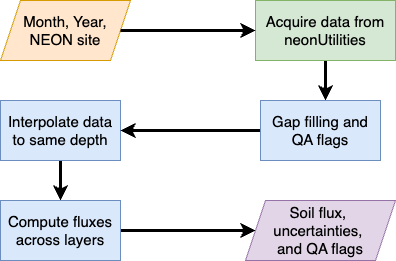
\includegraphics{figures/neonSoilFluxOutline.png}

}

\caption{\label{fig-package-diagram}Diagram of \texttt{neonSoilFlux} R
package. For a given month and NEON site, the package acquires all
relevant data to compute \(F_{S}\) using the \texttt{neonUtilities} R
package. Data are gap-filled according to reported QA flags and
interpolated to the same measurement depth before computing the soil
flux, uncertainties, and final QA flags.}

\end{figure}%

At a given NEON observation there are five different replicate soil
sensor arrays, with each sampling at five different soil depths
(Figure~\ref{fig-model-diagram}). The \texttt{neonSoilFlux} package
acquires measured soil water content (National Ecological Observatory
Network (NEON), 2024e), soil CO\(_{2}\) concentration (National
Ecological Observatory Network (NEON), 2024b), barometric pressure
(National Ecological Observatory Network (NEON), 2024a), soil
temperature (National Ecological Observatory Network (NEON), 2024d), and
soil properties (e.g.~bulk density) (National Ecological Observatory
Network (NEON), 2024c). The static soil properties are periodically
collected and assumed to be constant for the monthly observation period.

\begin{figure}

\centering{

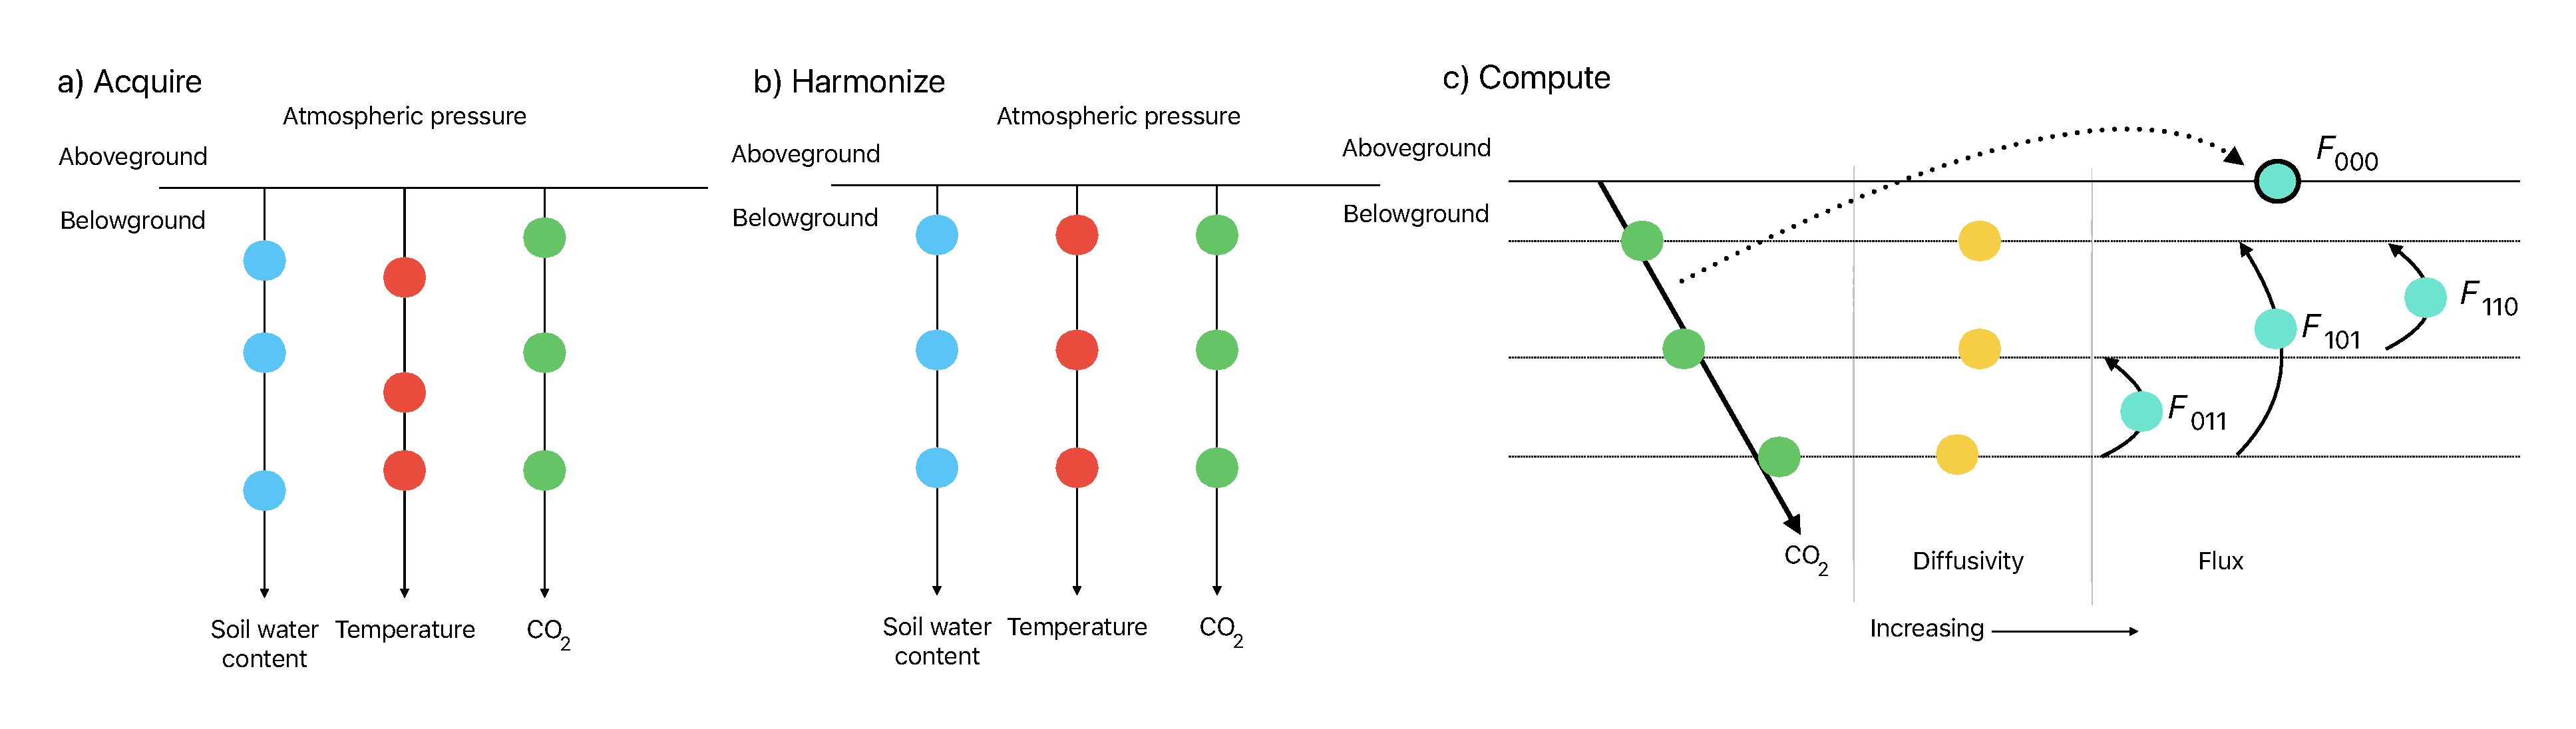
\includegraphics{figures/model-diagram.pdf}

}

\caption{\label{fig-model-diagram}Model diagram for data workflow for
the neonSoilFlux R package. a) Acquire: Data are obtained from given
NEON location and horizontal sensor location, which includes soil water
content, soil temperature, CO\(_{2}\) concentration, and atmospheric
pressure. All data are screened for quality assurance, with gap-filling
of missing data reported. b) Any belowground data are then harmonized to
the same depth as CO\(_{2}\) concentrations using linear regression. c)
The flux across a given depth is computed via Fick's law, denoted with
\(F_{ijk}\), where \(i\), \(j\), or \(k\) are either 0 or 1 denoting the
layer the flux is computed across (\(i\) = closest to surface, \(k\) =
deepest). The surface flux is all possible combinations of \(F_{ijk}\)
extrapolating the flux measurements to the surface, so \(F_{110}\) is
the surface flux intercept linearly extrapolating the measurements
\(F_{010}\) and \(F_{100}\).}

\end{figure}%

The workflow to computing a value of \(F_{S}\) with the
\texttt{neonSoilFlux} consists of three primary steps. First, NEON data
are acquired for a given site and month via the \texttt{neonUtilities} R
package (yellow parallelogram and green rectangle in
Figure~\ref{fig-package-diagram} and Panel a in
Figure~\ref{fig-model-diagram}). Acquired environmental data can be
exported to a comma separated value file for additional analysis.
Quality assurance (QA) flags with an observation are reported as an
indicator variable.

The next step is harmonizing the data to compute soil fluxes across soil
layers. This step consists of three different actions (blue rectangles
in Figure~\ref{fig-package-diagram} and Panel b in
Figure~\ref{fig-model-diagram}). If a given observation did is reported
as not passing a quality assurance check we applied a gap filling method
to replace that measurement with its monthly mean at that same depth
(Section~\ref{sec-gapfilling}). Belowground measurements of soil water
and soil temperature are then interpolated to the same depth as soil
CO\(_{2}\) measurements. The diffusivity
(Section~\ref{sec-compute-diffusivity}) and soil flux across different
soil layers (Section~\ref{sec-compute-soil-flux}) are then computed.

The final step is computing a surface soil flux through extrapolation to
the surface (purple parallelogram in Figure~\ref{fig-package-diagram}
and Panel c in Figure~\ref{fig-model-diagram}). Uncertainty on a soil
flux measurement is computed through quadrature. An aggregate QA flag
for each environmental measurement is also reported, representing if any
gap-filled measurements were used in the computation of a soil flux.
Within the soil flux-gradient method, several different approaches can
be used to derive a surface flux (Maier \& Schack-Kirchner, 2014); the
\texttt{neonSoilFlux} package reports eight different possible values of
soil surface flux (Section~\ref{sec-compute-soil-flux}).

\subsubsection{Gap-filling routine}\label{sec-gapfilling}

NEON reports QA flags as a binary value for a given measurement and
half-hourly time. We replaced any flagged measurements at a location's
spatial depth \(z\) with a bootstrapped sample of the monthly mean for
all un-flagged measurements for that month. hese measurements are
represented by the vector \(\mathbf{m}\), standard errors
\(\boldsymbol\sigma\), and the 95\% confidence interval (the so-called
expanded uncertainty, Farrance \& Frenkel (2012))
\(\boldsymbol\epsilon\). All of these vectors have length \(M\). We have
that \(\vec{\sigma}_{i}\leq\vec{\epsilon}_{i}\). We define the bias as
\(\mathbf{b}=\sqrt{\boldsymbol\epsilon^{2}-\boldsymbol\sigma^{2}}\).

We generate a vector of bootstrap samples of the distribution of the
monthly mean \(\overline{\boldsymbol{m}}\) and monthly standard error
\(\overline{\boldsymbol\sigma}\) the following ways:

\begin{enumerate}
\def\labelenumi{\arabic{enumi}.}
\tightlist
\item
  Randomly sample from the uncertainty and bias independently:
  \(\boldsymbol\sigma_{j}\) and the bias \(\mathbf{b}_{k}\) (not
  necessarily the same sample)
\item
  Generate a vector \(\mathbf{n}\) of length \(N\), where
  \(\mathbf{n}_{i}\) is a random sample from a normal distribution with
  mean \(\boldsymbol{m}_{i}\) and standard deviation
  \(\boldsymbol\sigma_{j}\). Since \(M<N\), values from \(\mathbf{m}\)
  will be reused.
\item
  With these \(N\) random samples,
  \(\overline{y}_{i}=\overline{\vec{x}}+\vec{b}_{k}\) and \(s_{i}\) is
  the sample standard deviation of \(\vec{x}\). We expect that
  \(s_{i} \approx \vec{\sigma}_{j}\).
\item
  The reported monthly mean and standard deviation are then computed
  \(\overline{\overline{y}}\) and \(\overline{s}\). Measurements and
  uncertainties that did not pass the QA check are then substituted with
  \(\overline{\overline{y}}\) and \(\overline{s}\).
\end{enumerate}

\subsubsection{Diffusivity computation}\label{sec-compute-diffusivity}

Soil diffusivity \(D_{a}\) at a given measurement depth is the product
of the diffusivity in free air \(D_{a,0}\) (m\(^{2}\) s\(^{-1}\)) and
the tortuosity \(\xi\) (no units) (Millington \& Shearer, 1971). Surface
barometric pressure (kPa) (National Ecological Observatory Network
(NEON), 2024a), soil temperature at depth (National Ecological
Observatory Network (NEON), 2024d), soil water content (National
Ecological Observatory Network (NEON), 2024e), and soil physical
properties (National Ecological Observatory Network (NEON), 2024c). Soil
physical properties are surveyed once at each site, whereas the other
measurements are provided on a half-hourly basis.

We compute \(D_{a,0}\) with Equation \ref{eq:da0}:

\begin{equation}
  D_{a,0} = 0.0000147 \cdot \left( \frac{T_{i} + 273.15}{293.15} \right)^{1.75} \cdot \left( \frac{P}{101.3} \right)
  \label{eq:da0}
\end{equation}

where \(T_{i}\) is soil temperature (\(^\circ\)C) at depth \(i\)
(National Ecological Observatory Network (NEON), 2024d) and \(P\)
surface barometric pressure (kPa) (National Ecological Observatory
Network (NEON), 2024a). At that soil depth, the tortuosity \(\xi\) is
defined by Equation \ref{eq:tortuosity} (Millington \& Shearer, 1971):

\begin{equation}
  \xi = \frac{(\phi - SWC_{i})^{10/3}}{\phi^{2}}
  \label{eq:tortuosity}
\end{equation}

In Equation \ref{eq:tortuosity}, \(SWC\) is the soil water content at
depth \(i\) (National Ecological Observatory Network (NEON), 2024e) and
\(\phi\) is the porosity (Equation \ref{eq:porosity}), which in turn is
a function of soil physical properties (National Ecological Observatory
Network (NEON), 2024c).

The tortuosity \(\xi\) is computed from soil porosity \(\phi\). :

\begin{equation}
  \phi = \left(1- \frac{\rho_{s}}{\rho_{m}} \right) \left(1-f_{V}\right)
  \label{eq:porosity}
\end{equation}

In Equation \ref{eq:porosity}, \(\rho_{m}\) is the particle density of
mineral soil (2.65 g cm\(^{-3}\)), \(\rho_{s}\) the soil bulk density (g
cm\(^{-3}\)) excluding coarse fragments greater than 2 mm (National
Ecological Observatory Network (NEON), 2024c). The term \(f_{V}\) is a
site-specific value that accounts for the proportion of soil fragments
between 2-20 mm. Soil fragments greater than 20 mm were not estimated
due to limitations in the amount of soil that can be analyzed (National
Ecological Observatory Network (NEON), 2024c). We assume there are no
pores within rocks. Values of \(\rho_{s}\), \(\rho_{m}\) are assumed to
be constant across the soil profile and the same at each site sampling
location.

\subsubsection{Soil flux computation}\label{sec-compute-soil-flux}

We applied Fick's law (Equation \ref{eq:ficks}) to compute the soil flux
\(F_{ij}\) (\(\mu\)mol m\(^{-2}\) s\(^{-1}\)) across two adjacent soil
depths \(i\) and \(j\):

\begin{equation}
  F_{ij} = -D_{a} \frac{dC}{dz}
  \label{eq:ficks}
\end{equation}

where \(D_{a}\) is the diffusivity (m\(^{2}\) s\(^{-1}\)) and
\(\frac{dC}{dz}\) is the gradient of CO\(_{2}\) molar concentration
(\(\mu\)mol m\(^{-3}\), so the gradient has units of \(\mu\)mol
m\(^{-3}\) m\(^{-1}\)). The diffusivity (described below) is a function
of soil temperature, soil water content, and soil physical properties.
The soil surface flux is theoretically defined by applying Equation
\ref{eq:ficks} to measurements collected at the soil surface and
directly below the surface. Measurements of soil temperature, soil water
content, and soil CO\(_{2}\) molar concentration across the soil profile
allow for application of Equation \ref{eq:flux} across different soil
depths. The flux gradient method approximates the soil surface flux
either by (1) extrapolation of Equation \ref{eq:ficks} across
sub-surface measurement depths to the surface, typically assuming soil
flux is a linear function of depth (Maier \& Schack-Kirchner, 2014) or
(2) linear extrapolation of \(D_{a}\) to the surface and from direct
calculation of \(\frac{dC}{dz}\) from the CO\(_{2}\) profile. All these
approaches are pThe \texttt{neonSoilFlux} package provides several
different methods to compute \(F_{s}\) for the end-user to compare.

\subsubsection{Reporting of surface
fluxes}\label{reporting-of-surface-fluxes}

A surface flux estimate is derived from Fick's Law (Equation
\ref{eq:ficks}), which is the product of a diffusivity and a CO\(_{2}\)
concentration gradient (Maier \& Schack-Kirchner, 2014). The
\texttt{neonSoilFlux} package provides eight different surface flux
estimates, which represent different considerations of how Fick's Law is
applied. First, we apply simple linear regression to both CO\(_{2}\) and
\(D_{a}\) at the three different measurement depths. Next, the slope and
intercept (and uncertainty by quadrature) from these regressions are
used to compute a suite of eight different surface flux estimates
(denoted by \(F_{ijk}\)):

\begin{itemize}
\tightlist
\item
  \(F_{000}\) is a surface flux estimate using the intercept of the
  linear regression of \(D_{a}\) and the slope from linear regression of
  CO\(_{2}\) (which represents \(\frac{dC}{dz}\) in Fick's Law). Tang et
  al. (2003) used this approach to compute fluxes in an oak-grass
  savannah.
\item
  \(F_{010}\), \(F_{001}\) are fluxes across the two most shallow layers
  and two deepest layers respectively. The diffusivity used in Fick's
  Law is always at the deeper measurement layer. When used as a surface
  flux estimate we assume CO\(_{2}\) remains constant above this flux
  depth.
\item
  \(F_{100}\) is a flux estimate where the gradient \(\frac{dC}{dz}\) is
  estimated using the intercept from linear regression of CO\(_{2}\) and
  the top measurement depth for CO\(_{2}\). The diffusivity used in
  Fick's Law is always at the first measurement layer. de Jong \&
  Schappert (1972) applied this approach in a Canadian prairie.
\item
  \(F_{110}\), \(F_{101}\), \(F_{011}\) are a surface flux estimates
  using linear extrapolation between \(F_{100}\) and \(F_{010}\);
  \(F_{100}\) and \(F_{001}\); or \(F\_{010}\) and \(F_{001}\)
  respectively. Hirano et al. (2003) and Tang et al. (2005) used an
  approach similar to \(F_{101}\) in a temperate deciduous broadleaf
  forest and ponderosa pine forest respectively.
\item
  \(F_{111}\) is a surface flux estimate using linear extrapolation
  between \(F_{100}\), \(F_{010}\), and \(F_{001}\).
\end{itemize}

Uncertainty in all \(F_{ijk}\) is computed through quadrature.

\subsection{Post processing
evaluation}\label{post-processing-evaluation}

Following collection of field measurements from the LICOR and
calculation of the soil fluxes from \texttt{neonSoilFlux} package, we
compared measured soil fluxes (from the LICOR instruments) to a given
soil flux calculation during the same half hour. At each site and flux
compuation method we also computed the R\(^{2}\) value for the
half-hourly and measured LICOR values and the RMSE.

We evaluate the efficacy of results from the flux-gradient method in two
ways. First, we calculated the signal to noise ratio (SNR), defined as
the ratio of the reported flux to its uncertainty
(\(F_{ijk}/\sigma_{ijk}\)).

We evaluated if the measured field fluxes were within the calculated
uncertainty from the flux-gradient method using the various approaches
outlined above. We observed that the calculated quadrature uncertainty
in many cases can be much larger than the reported measurement (as shown
through the signal to noise ratio, SNR = \(F_{ijk}/\sigma_{ijk}\). We
evaluated \(| F_{S} - F_{ijk} | < (1-\epsilon) \sigma_{ijk}\), where
\(F_{S}\) is a measured field soil flux from the LICOR 6800 (the LICOR
8250 was used at only three sites) and \(F_{ijk}\) is a computed flux
method from the flux-gradient, and \(\sigma_{ijk}\) is the reported
uncertainty for the flux method. The parameter \(\epsilon\) was an
uncertainty reduction factor to evaluate how sensitive the results were
given, measured by the proportion of field measurements contained in
that range.

\subsection{Diffusivity back
calculations}\label{diffusivity-back-calculations}

We also computed the diffusivity at each of the different sites from the
derived flux values and the reported gradient in CO2 at each of the
surface layers (Figure XXXX) through dividing \(F_{field}/dC/dz\) These
values were then compared to reported diffusivity from the flux
computation method.

Finally, the bulk density at a given site was then also computed through
back calculation.

\section{Results}\label{results}

Figure~\ref{fig-flux-results} reports out the measured fluxes from the
LICOR 6800 and 8250 and computed fluxes and uncertainty at each
measurement site. Results are reported in local time. Positive values of
the flux indicate that there is a flux moving towards the surface (FIX
WRITING) For ease of clarity the fluxes at \(F_{111}\) and \(F_{000}\)
are only shown in the top row (surface), followed by the fluxes at
individual separate layer (\(F_{100}\), \(F_{010}\), \(F_{001}\)).
Overall, with the exception of WREF and SRER (discussed later) the
computed fluxes were on the same order of magnitude and timing as the
measured field fluxes.

\begin{figure}

\centering{

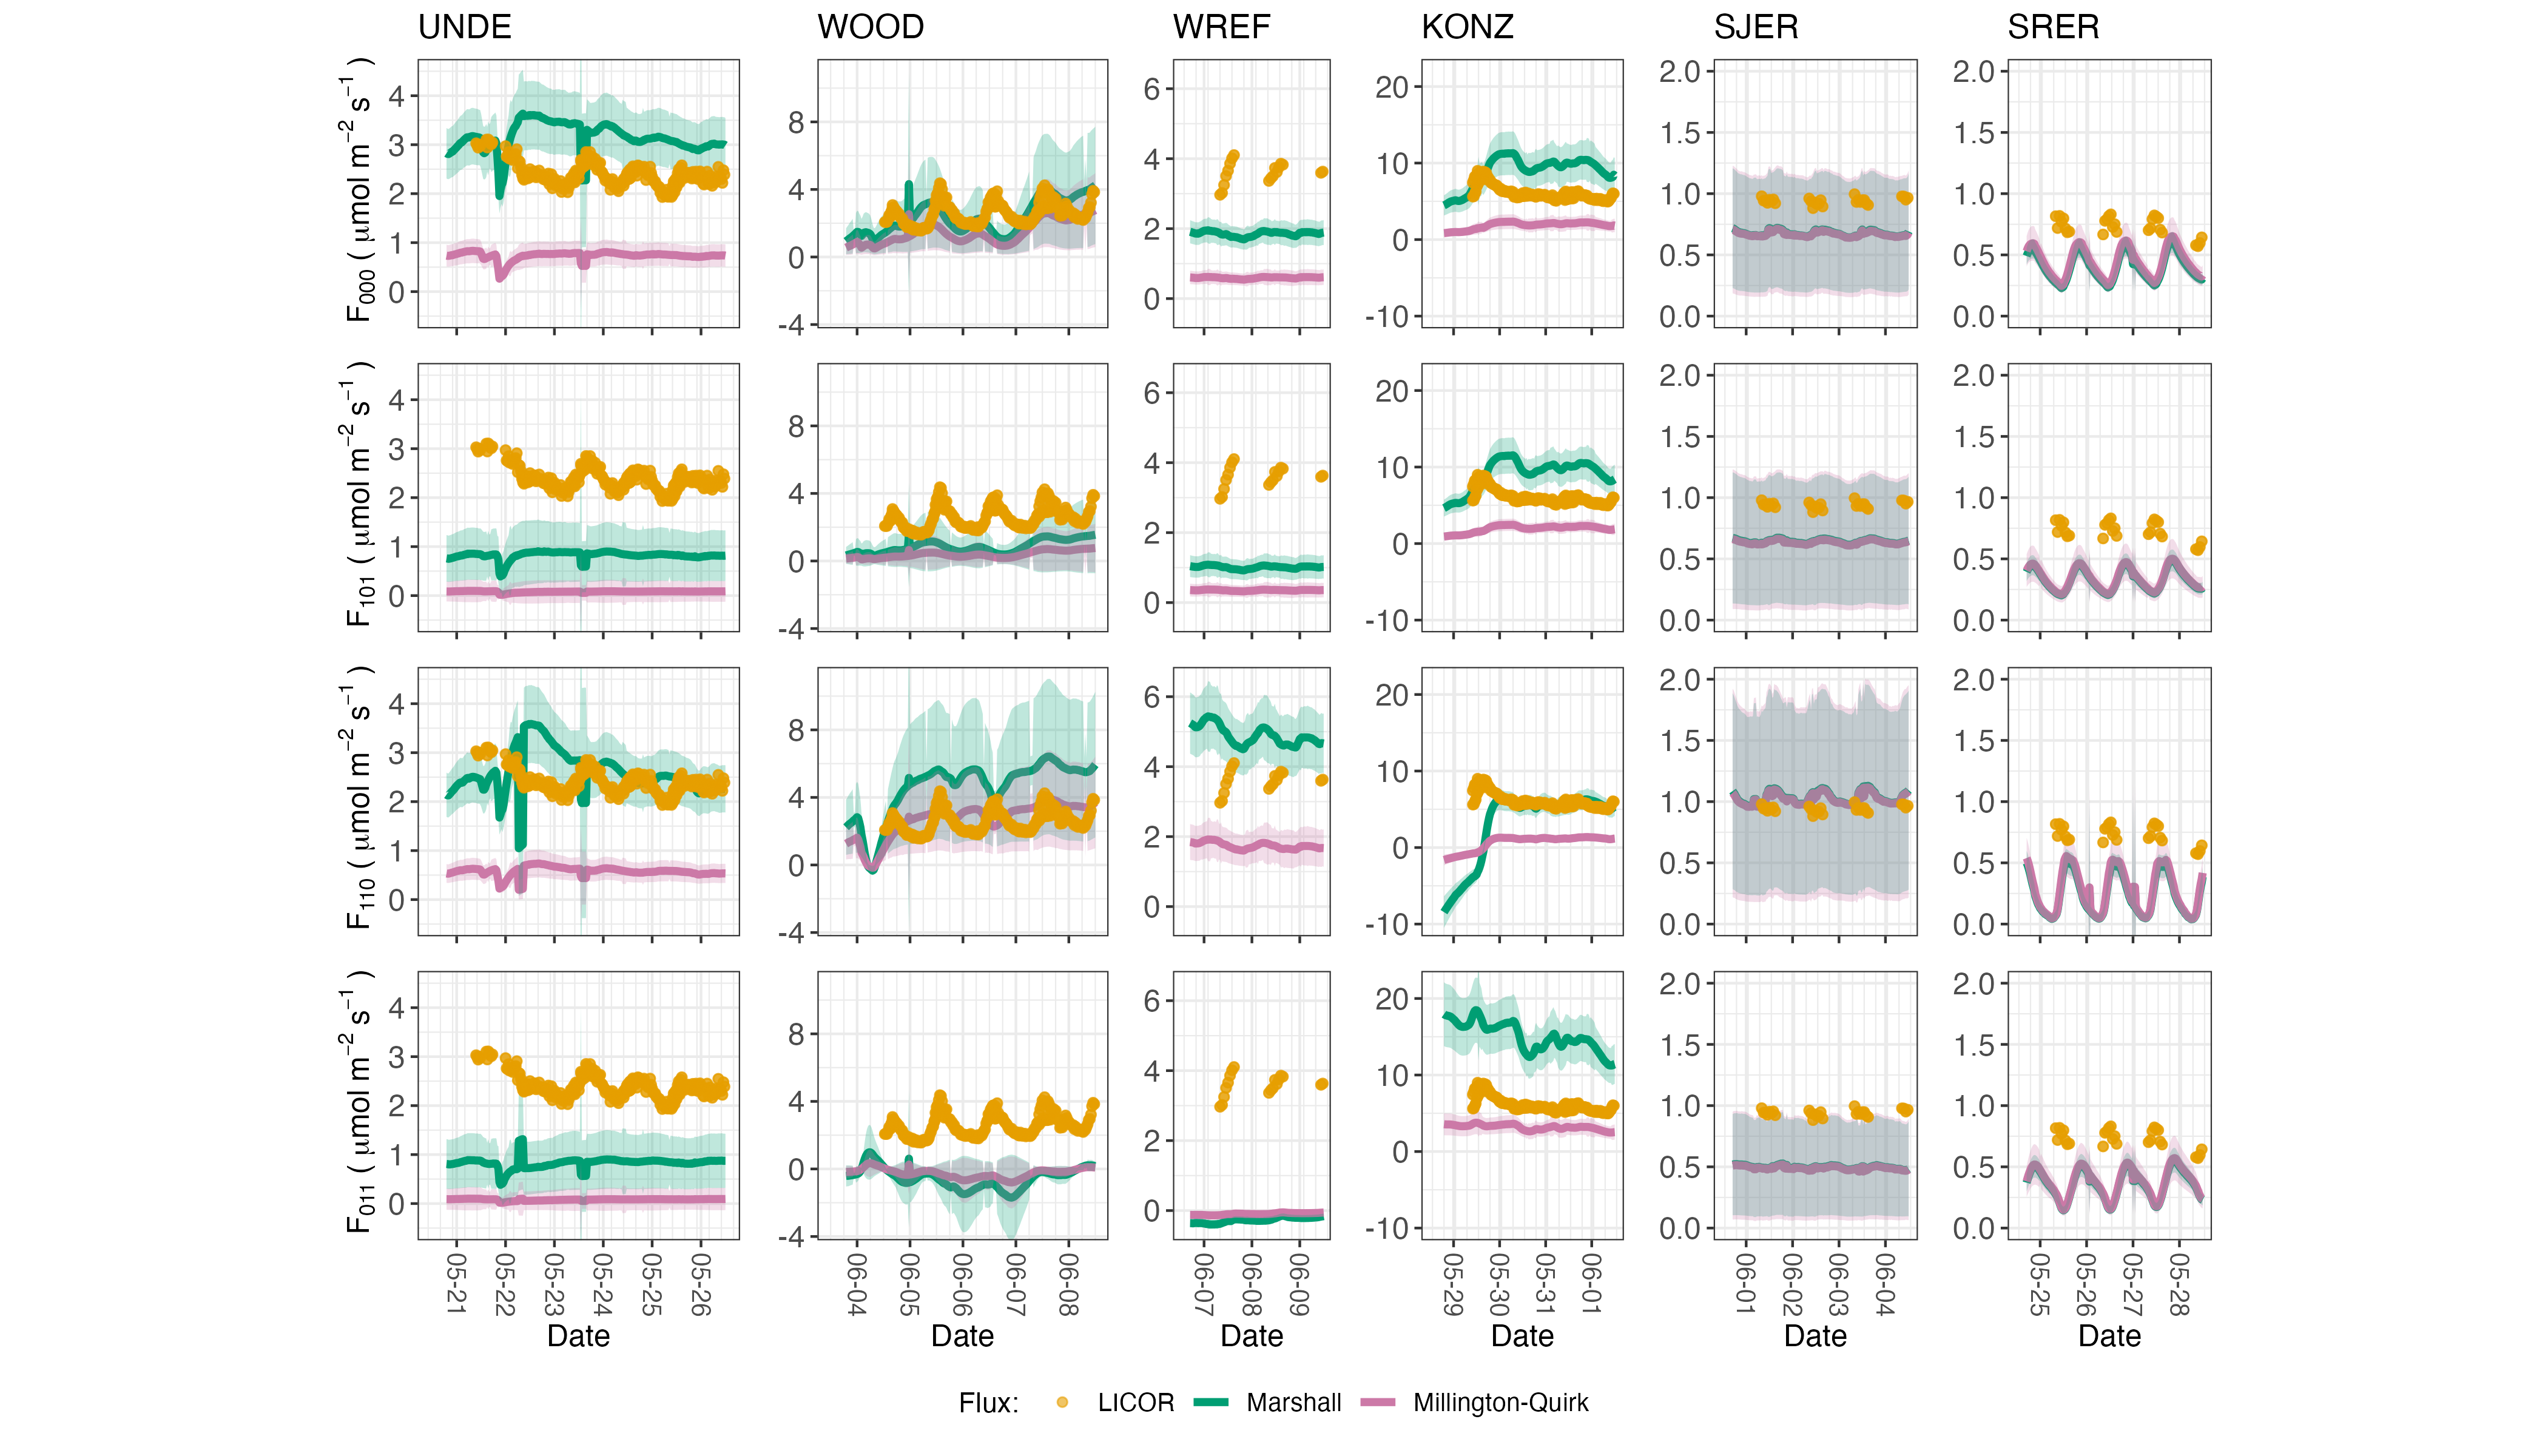
\includegraphics{figures/flux-results.png}

}

\caption{\label{fig-flux-results}Results for different flux
computations, organized by site (in increasing temperature show at each
site) across different measurement levels. \(F_{000}\) comes from the
diffusivity extrapolation and \(F_{111}\) extrapolation across the
surface. Field measurements are shown at the top of each plot. The
computed flux values are shown with reported uncertainty as well.}

\end{figure}%

Figure~\ref{fig-gap-filled-stats} reports which environmental
measurements at each site relied on gap-filled measurements (left plot)
and in the aggregate, the total number of gap-filled measurements used
for each half-hourly flux computation. the largest contribution to
gap-filled data was soil water followed by soil temperature.

\begin{figure}

\centering{

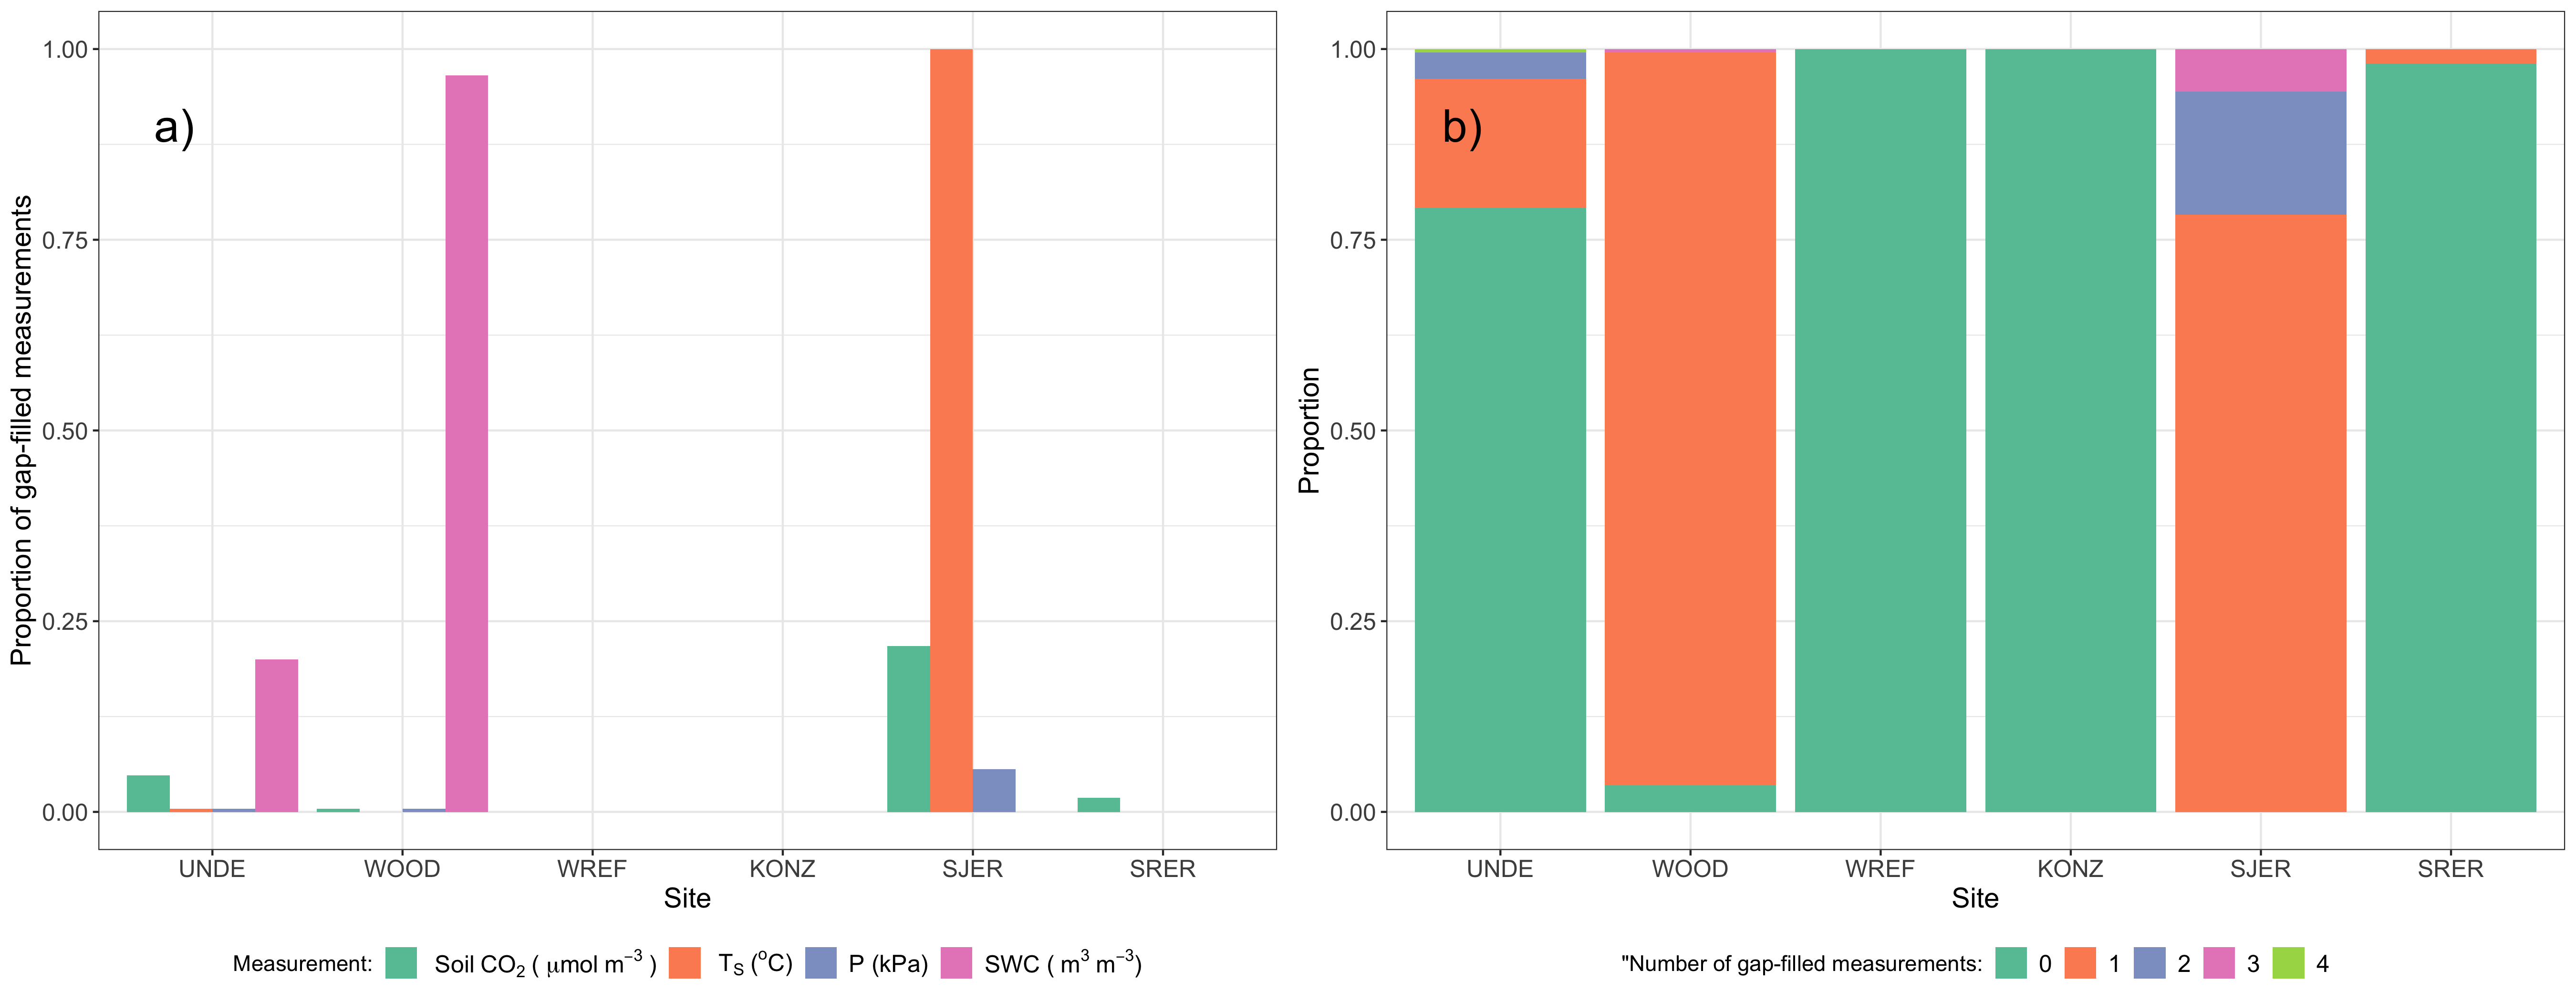
\includegraphics{figures/gap-filled-stats.png}

}

\caption{\label{fig-gap-filled-stats}Left panel: Proportion of
gap-filled environmental observations at each site. Right panel:
proportion of measurements that used gap-filled environmental data (0 -
4) at each site. BLAH}

\end{figure}%

\begin{figure}

\centering{

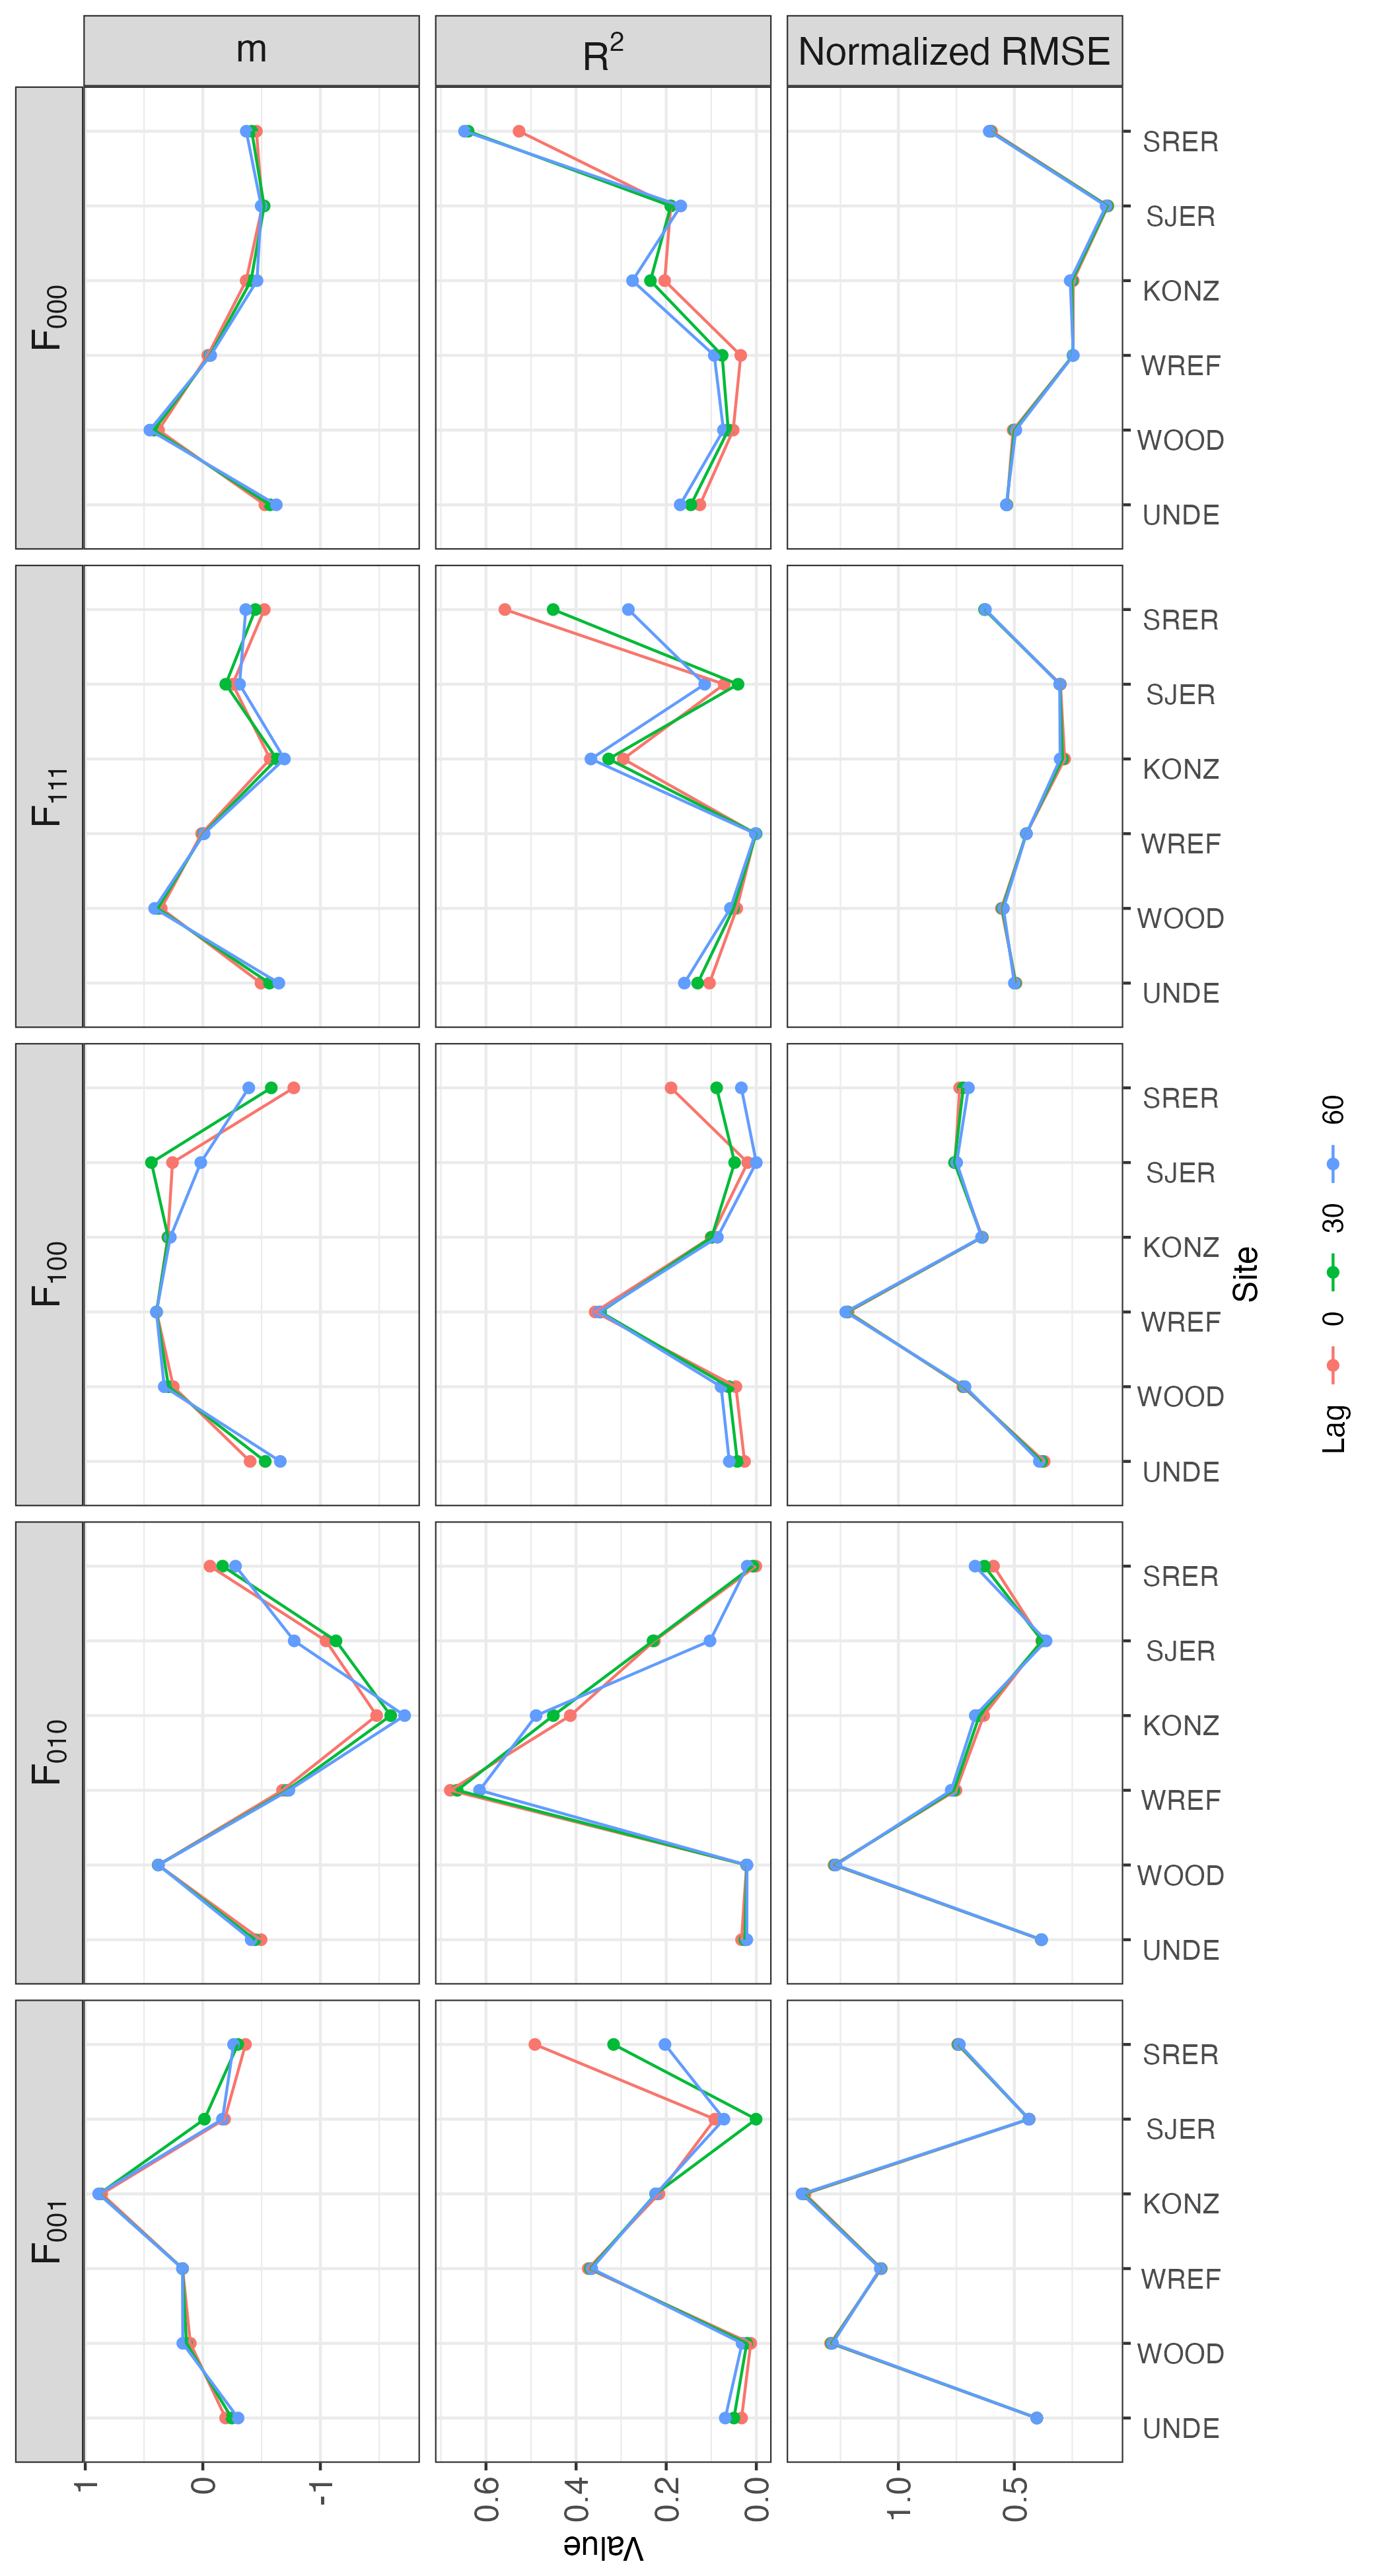
\includegraphics{figures/stats-plot.png}

}

\caption{\label{fig-stats-plot}}

\end{figure}%

Figure: flux results at the different levels (000,111,001,010,100)
Diffusivity at the different levels for comparison (also include derived
diffusivity?) Stats at the different levels (with the lags)

LEAD IN TABLE HERE These results are reported in
Figure~\ref{fig-uncertainty-stats}.

\begin{figure}

\centering{

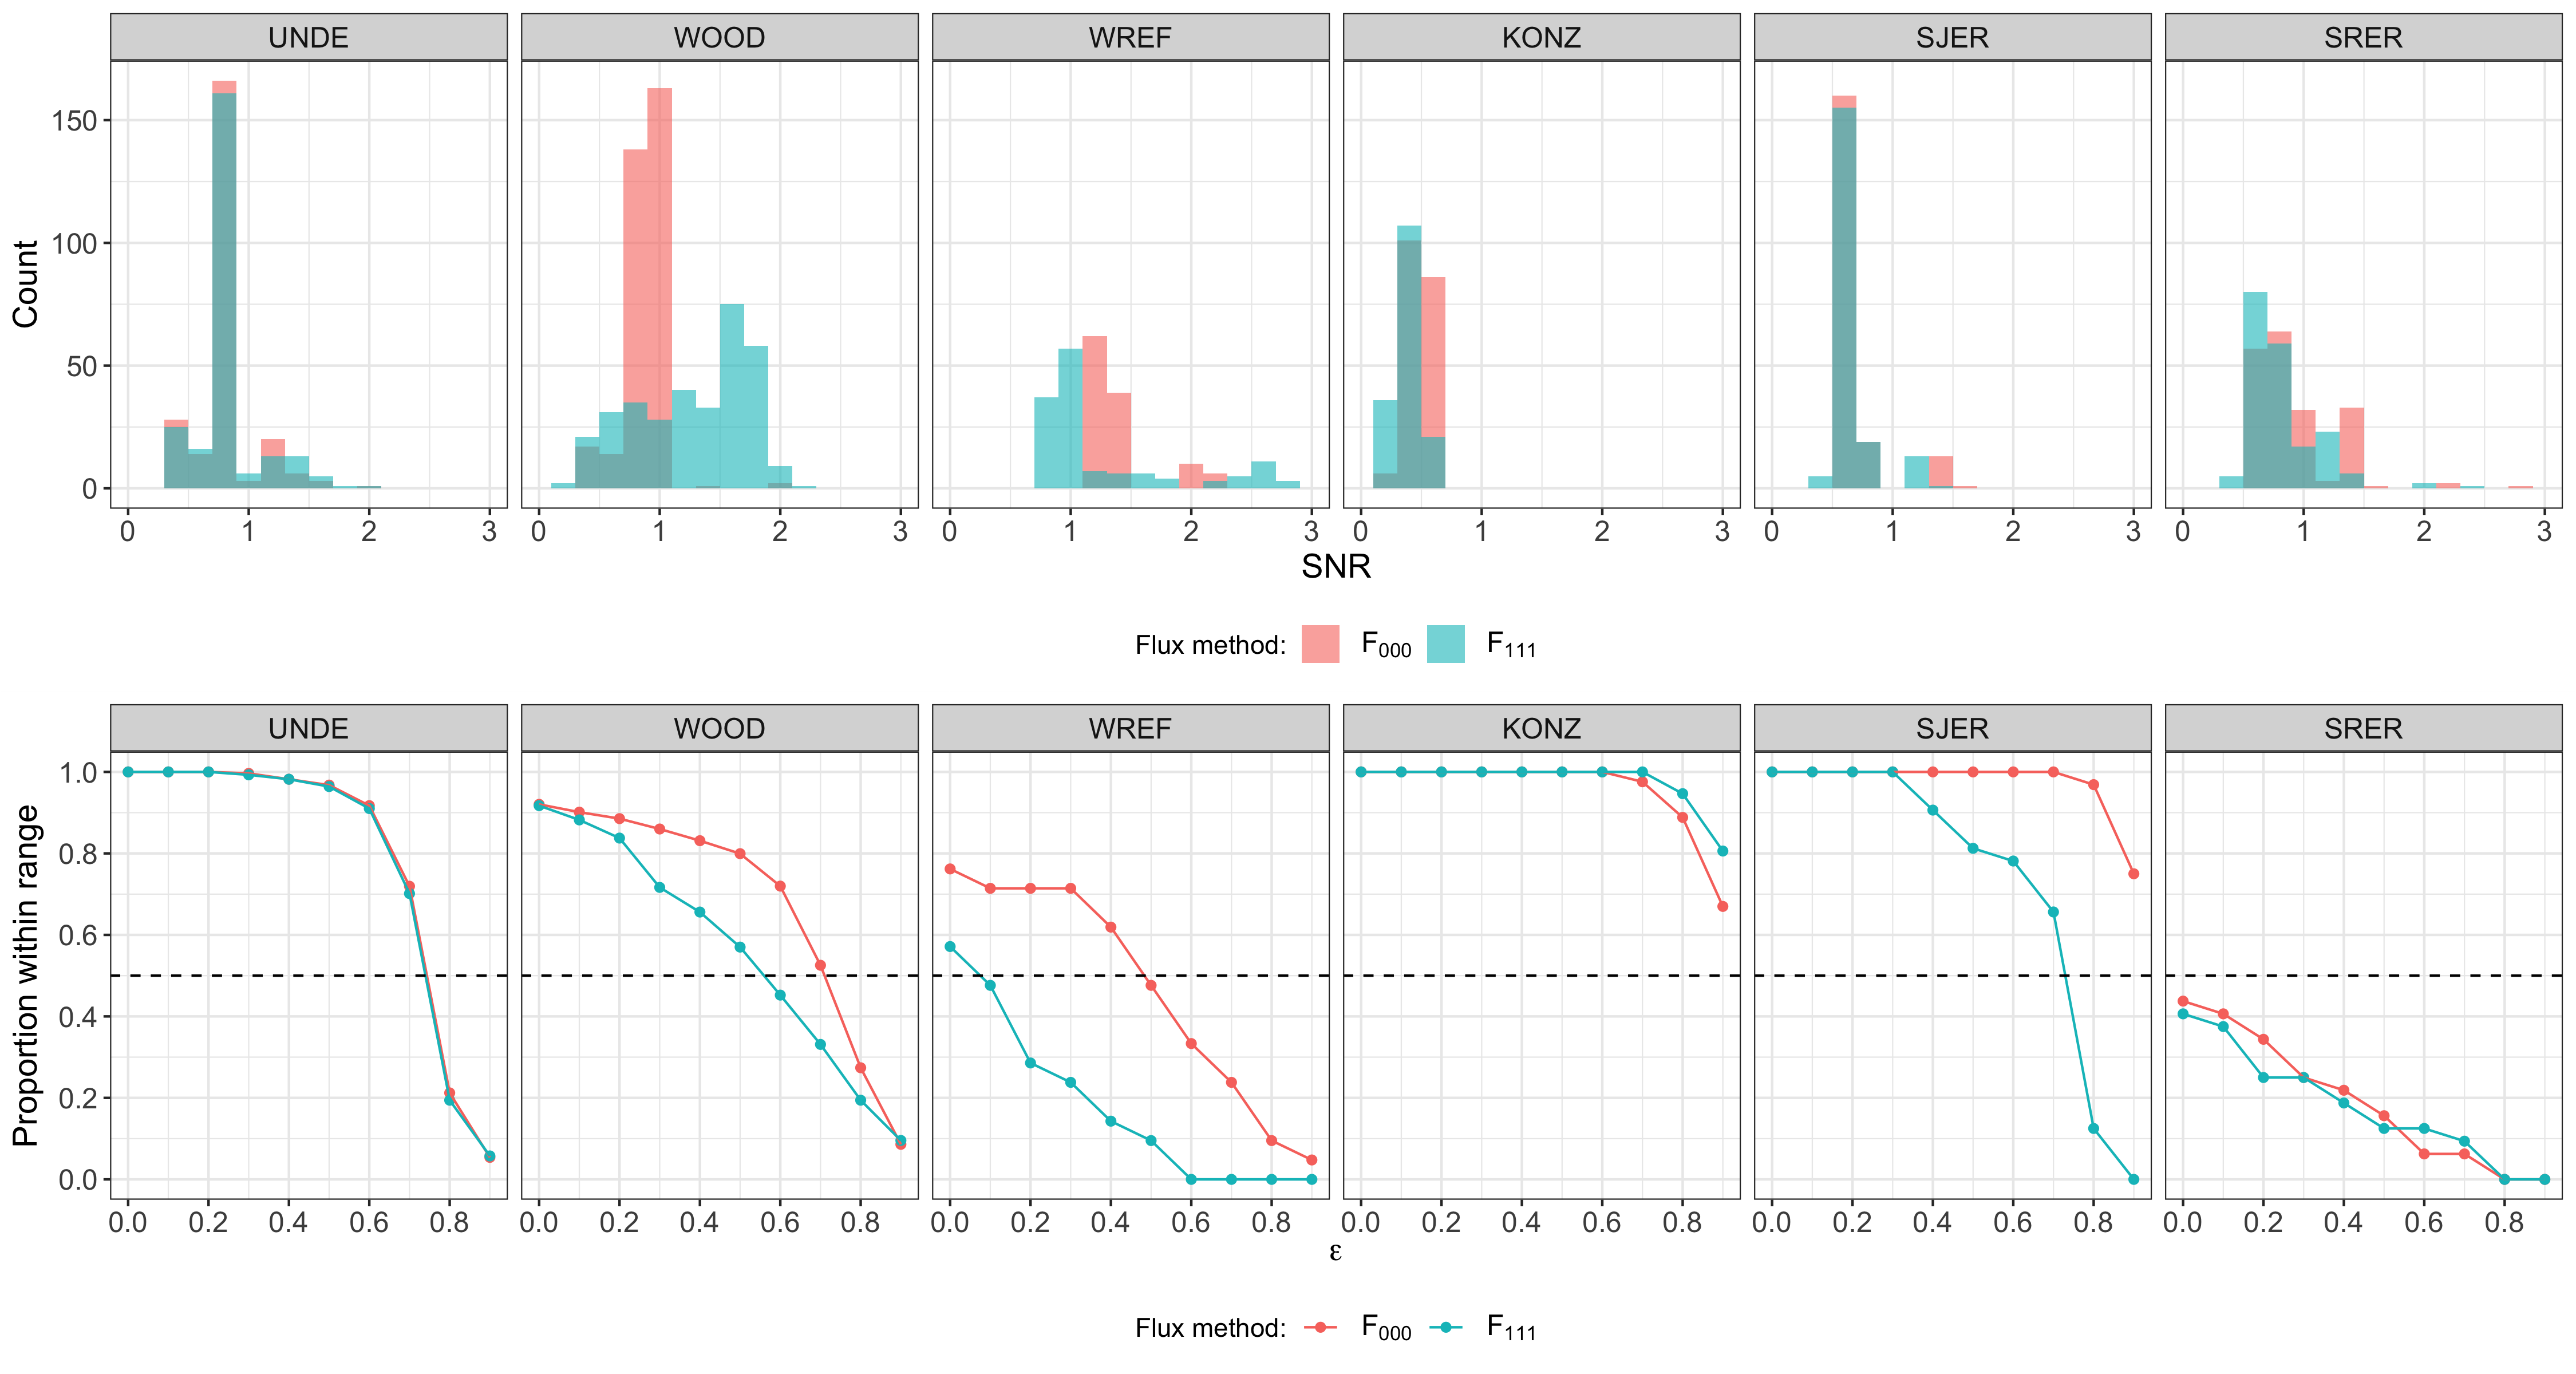
\includegraphics{figures/uncertainty-stats.png}

}

\caption{\label{fig-uncertainty-stats}Top panel: distribution of SNR
values across each of the different sites for the \(F_{000}\) and
\(F_{111}\) flux gradient calculations. Bottom panel: Computation of
uncertainty reduction to evaluate. As \(\epsilon\) increases this
indicates that the uncertainty estimate reduces, making it harder to be
within the range. BLAH}

\end{figure}%

Calculated diffusivity from both the \texttt{neonSoilFlux} method and
back calculated from the LICOR are reported in Figure
Figure~\ref{fig-diffusivity-plot}. SAY MORE

\begin{figure}

\centering{

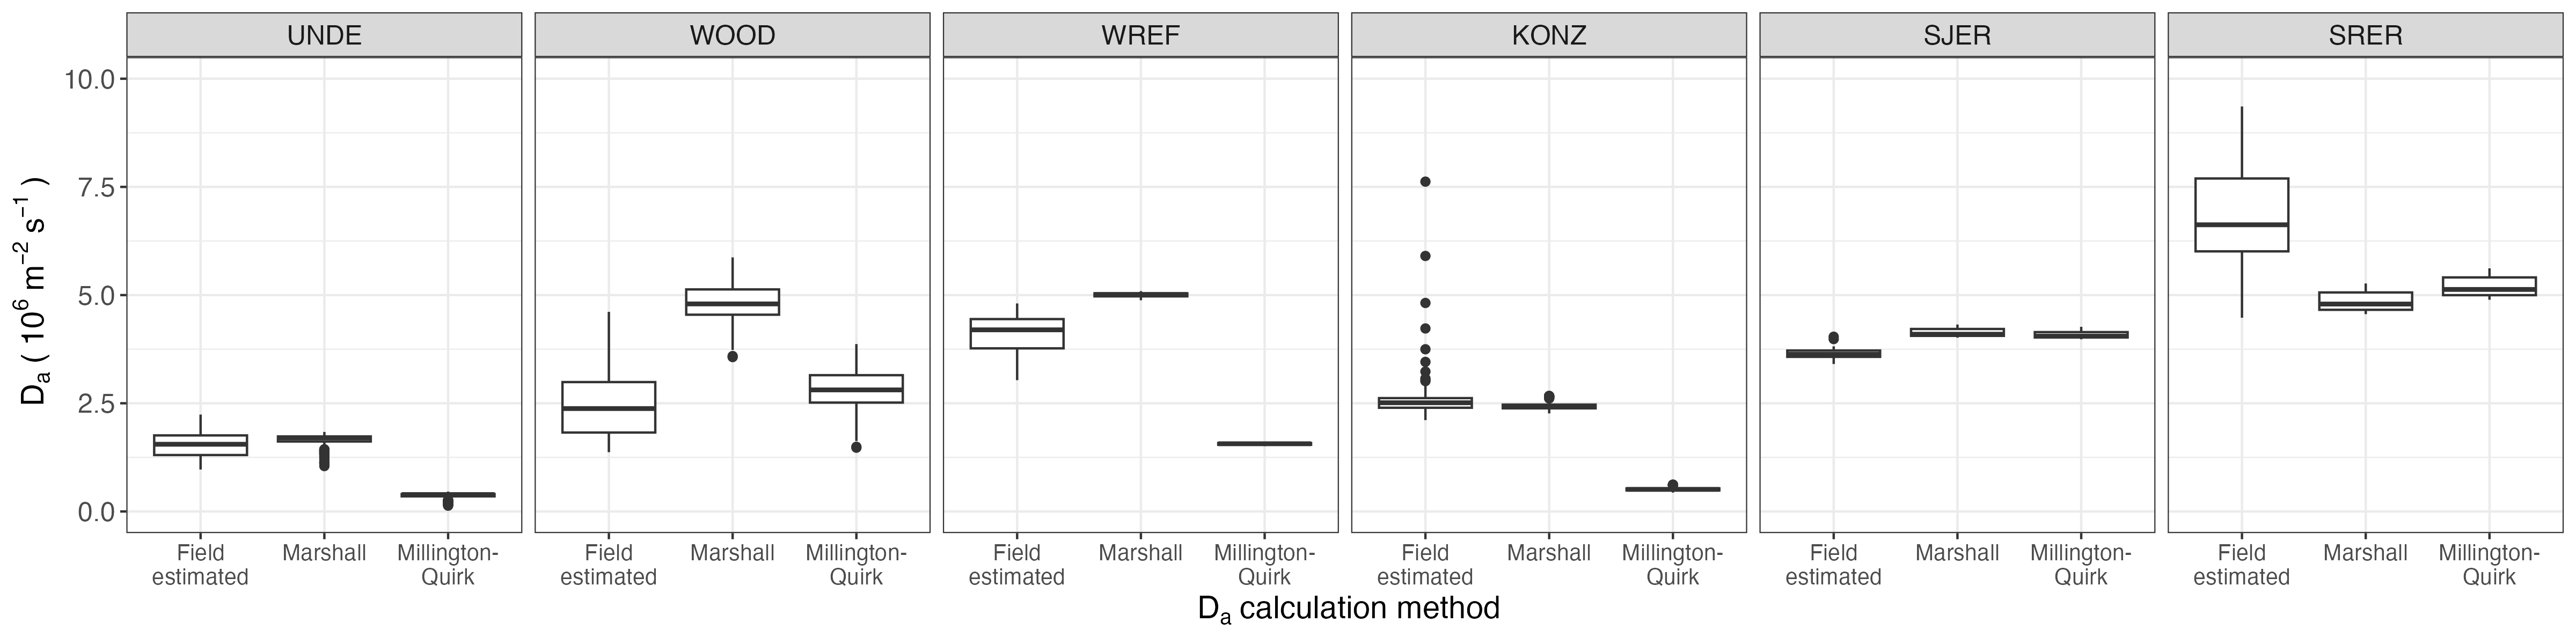
\includegraphics{figures/diffusivity-plot.png}

}

\caption{\label{fig-diffusivity-plot}Calculation of diffusivity at each
of the sites SAY MORE}

\end{figure}%

\section{Discussion}\label{discussion}

Our core goals in this study were: 1) to generate estimates of soil flux
from continuous soil sensor data at terrestrial NEON sites using the
flux-gradient method and then 2) to compare those estimates to
field-measured fluxes based on the closed chamber approach at six focal
sites spanning six different states.

We were able to show that the flux-gradient method produced estimates
within XX of the field measured values at X of Y sites.

In developing and validating our approach, we faced a number of
challenges related to data availability and uncertainty,
including\ldots{} gap filling, sensor calibration, depth interpolation,
rainstorms, etc

These challenges notwithstanding, the method used here and made
available in the \texttt{neonSoilFlux} R package is able to produce
nearly continuous estimates of flux across all XXYY terrestrial NEON
sites. These estimates are a significant improvement on available
approaches to constrain the portion of ecosystem respiration
attributable to the soil. This, in turn, aids in our ability to
understand the components of net ecosystem flux assessed at these sites
using the co-located eddy flux towers.

This study presents a unified data science workflow to efficiently
process automated measurements of belowground soil CO\(_{2}\)
concentrations, water, and temperature to infer estimates of soil
effluxes through application of Fick's Law. Derived results from the
\texttt{neonSoilFlux} package have patterns that are consistent, and
comparable, to those directly measured to the field (Figure XXX). The
advantage to the \texttt{neonSoilFlux} package is the calculation of
fluxes across different measurement depths, allowing for additional
site-specific customization. Here application of the flux-gradient
method provides a baseline estimate of soil fluxes that could be
complemented through additional field measurements (e.g.~LICOR).

The largest source of uncertainty to improve reliability of the flux
estimate is to prevent the usage of gap-filled data, especially with
soil water (Figure XXX). Across the observed half-hourly periods for
field measurements, the percentage of half-hourly periods where all four
environmental measurements were available spanned from 0\% (SJER) to 7\%
(SRER), but three sites (WREF, SRER, UNDE) had 95\% of half-hourly
intervals with just one gap-filled measurement.Where appropriate we have
replaced measurements flagged to the protocol with a monthly gap-filled
value. Further extensions of the gapfilling method could use more
sophisticated gap-filling routines, similar to what is used for net
ecosystem carbon exchange (Falge et al., 2001; Liu et al., 2023;
Mariethoz et al., 2015; Moffat et al., 2007; Zhang et al., 2023).

The \texttt{neonSoilFlux} package provides eight different approaches of
values for a soil flux. We believe these approaches reflect a variety of
site-specific determination and assumptions used to generate a soil flux
measurement (Maier \& Schack-Kirchner, 2014), with the choice of method
having a determinative approach on reported values. Reported results
could further be distilled down using ensemble averaging averaging
approaches (Elshall et al., 2018; Raftery et al., 2005).

Figures XXX suggests that the provided uncertainty from
\texttt{neonSoilFlux} is an overestimate compared to what is actually
computed. When \(\epsilon=0\) in Figure
Figure~\ref{fig-uncertainty-stats}, that means we are just using the
reported uncertainty from neonSoilFlux. Looking at that (epsilon = 0)
shows field measurements UNDE, KONZ, SJER are 100\% within the reported
intervals from neonSoilFlux. But those sites tend to have a SNR
\textless{} 1, so the uncertainty is pretty noisy. For UNDE, we could
even reduce the uncertainty by a factor of 75\% (epsilon = 0.75), more
than half of the field measurements will still be within the reported
intervals. For KONZ, we are still within 70\% of the reported intervals
when uncertainty is reduced by 90\%. To me, that suggests that while the
reported accuracy (as compared to field measurements), we do have higher
precision.

Diffusivity taken from the megapit. Big microsite and temporal
differences, soil shrink / swell. How do we think about what that means
for using this approach to generalize across a NEON site over continuous
time.

\begin{itemize}
\tightlist
\item
  Back calculation of bulk density to NEON sites.
\end{itemize}

\section{Conclusions}\label{conclusions}

\section{Acknowledgments}\label{acknowledgments}

\section{Conflict of Interest
Statements}\label{conflict-of-interest-statements}

\section*{Author Contributions}\label{author-contributions}
\addcontentsline{toc}{section}{Author Contributions}

\phantomsection\label{refs}
\begin{CSLReferences}{1}{0}
\bibitem[\citeproctext]{ref-baldocchiMeasuringFluxesTrace2014}
Baldocchi, D. (2014). Measuring fluxes of trace gases and energy between
ecosystems and the atmosphere - the state and future of the eddy
covariance method. \emph{Global Change Biology}, \emph{20}(12),
3600--3609. \url{https://doi.org/10.1111/gcb.12649}

\bibitem[\citeproctext]{ref-berenbaumReportNSFBIO2015}
Berenbaum, M. R., Carpenter, S. R., Hampton, S. E., Running, S. W., \&
Stanzione, D. C. (2015). \emph{Report from the {NSF BIO Advisory
Committee Subcommittee} on {NEON Scope Impacts}}.

\bibitem[\citeproctext]{ref-bond-lambertyNewTechniquesData2018}
Bond-Lamberty, B. (2018). New {Techniques} and {Data} for
{Understanding} the {Global Soil Respiration Flux}. \emph{Earth's
Future}, \emph{6}(9), 1176--1180.
\url{https://doi.org/10.1029/2018EF000866}

\bibitem[\citeproctext]{ref-bond-lambertyTwentyYearsProgress2024}
Bond-Lamberty, B., Ballantyne, A., Berryman, E., Fluet-Chouinard, E.,
Jian, J., Morris, K. A., Rey, A., \& Vargas, R. (2024). Twenty {Years}
of {Progress}, {Challenges}, and {Opportunities} in {Measuring} and
{Understanding Soil Respiration}. \emph{Journal of Geophysical Research:
Biogeosciences}, \emph{129}(2), e2023JG007637.
\url{https://doi.org/10.1029/2023JG007637}

\bibitem[\citeproctext]{ref-bond-lambertyCOSORECommunityDatabase2020}
Bond-Lamberty, B., Christianson, D. S., Malhotra, A., Pennington, S. C.,
Sihi, D., AghaKouchak, A., Anjileli, H., Altaf Arain, M., Armesto, J.
J., Ashraf, S., Ataka, M., Baldocchi, D., Andrew Black, T., Buchmann,
N., Carbone, M. S., Chang, S.-C., Crill, P., Curtis, P. S., Davidson, E.
A., \ldots{} Zou, J. (2020). {COSORE}: {A} community database for
continuous soil respiration and other soil-atmosphere greenhouse gas
flux data. \emph{Global Change Biology}, \emph{26}(12), 7268--7283.
\url{https://doi.org/10.1111/gcb.15353}

\bibitem[\citeproctext]{ref-bond-lambertyGlobalDatabaseSoil2010}
Bond-Lamberty, B., \& Thomson, A. (2010). A global database of soil
respiration data. \emph{Biogeosciences}, \emph{7}(6), 1915--1926.
\url{https://doi.org/10.5194/bg-7-1915-2010}

\bibitem[\citeproctext]{ref-bond-lambertyGlobalRelationshipHeterotrophic2004}
Bond-Lamberty, B., Wang, C., \& Gower, S. T. (2004). A global
relationship between the heterotrophic and autotrophic components of
soil respiration? \emph{Global Change Biology}, \emph{10}(10),
1756--1766. \url{https://doi.org/10.1111/j.1365-2486.2004.00816.x}

\bibitem[\citeproctext]{ref-chenDoesGeneralTemperatureDependent2005}
Chen, H., \& Tian, H.-Q. (2005). Does a {General Temperature-Dependent
Q10 Model} of {Soil Respiration Exist} at {Biome} and {Global Scale}?
\emph{Journal of Integrative Plant Biology}, \emph{47}(11), 1288--1302.
\url{https://doi.org/10.1111/j.1744-7909.2005.00211.x}

\bibitem[\citeproctext]{ref-davidsonVariabilityRespirationTerrestrial2006}
Davidson, E. A., Janssens, I. A., \& Luo, Y. (2006). On the variability
of respiration in terrestrial ecosystems: Moving beyond {Q10}.
\emph{Global Change Biology}, \emph{12}, 154--164.
\url{https://doi.org/10.1111/j.1365-2486.2005.01065.x}

\bibitem[\citeproctext]{ref-dejongCalculationSoilRespiration1972}
de Jong, E., \& Schappert, H. J. V. (1972). Calculation of {Soil
Respiration} and {Activity} from {CO2 Profiles} in the {Soil}.
\emph{Soil Science}, \emph{113}(5), 328--333.

\bibitem[\citeproctext]{ref-desaiDriversDecadalCarbon2022}
Desai, A. R., Murphy, B. A., Wiesner, S., Thom, J., Butterworth, B. J.,
Koupaei-Abyazani, N., Muttaqin, A., Paleri, S., Talib, A., Turner, J.,
Mineau, J., Merrelli, A., Stoy, P., \& Davis, K. (2022). Drivers of
{Decadal Carbon Fluxes Across Temperate Ecosystems}. \emph{Journal of
Geophysical Research: Biogeosciences}, \emph{127}(12), e2022JG007014.
\url{https://doi.org/10.1029/2022JG007014}

\bibitem[\citeproctext]{ref-elshallRelativeModelScore2018}
Elshall, A. S., Ye, M., Pei, Y., Zhang, F., Niu, G.-Y., \&
Barron-Gafford, G. A. (2018). Relative model score: A scoring rule for
evaluating ensemble simulations with application to microbial soil
respiration modeling. \emph{Stochastic Environmental Research and Risk
Assessment}, \emph{32}(10), 2809--2819.
\url{https://doi.org/10.1007/s00477-018-1592-3}

\bibitem[\citeproctext]{ref-falgeGapFillingStrategies2001}
Falge, E., Baldocchi, D., Olson, R., Anthoni, P., Aubinet, M.,
Bernhofer, C., Burba, G., Ceulemans, R., Clement, R., Dolman, H.,
Granier, A., Gross, P., Grünwald, T., Hollinger, D., Jensen, N.-O.,
Katul, G., Keronen, P., Kowalski, A., Lai, C. T., \ldots{} Wofsy, S.
(2001). Gap filling strategies for defensible annual sums of net
ecosystem exchange. \emph{Agricultural and Forest Meteorology},
\emph{107}(1), 43--69.
\url{https://doi.org/10.1016/S0168-1923(00)00225-2}

\bibitem[\citeproctext]{ref-farranceUncertaintyMeasurementReview2012}
Farrance, I., \& Frenkel, R. (2012).
\href{https://www.ncbi.nlm.nih.gov/pmc/articles/PMC3387884}{Uncertainty
of {Measurement}: {A Review} of the {Rules} for {Calculating Uncertainty
Components} through {Functional Relationships}}. \emph{The Clinical
Biochemist Reviews}, \emph{33}(2), 49--75.

\bibitem[\citeproctext]{ref-friedlingsteinGlobalCarbonBudget2023}
Friedlingstein, P., O'Sullivan, M., Jones, M. W., Andrew, R. M., Bakker,
D. C. E., Hauck, J., Landschützer, P., Le Quéré, C., Luijkx, I. T.,
Peters, G. P., Peters, W., Pongratz, J., Schwingshackl, C., Sitch, S.,
Canadell, J. G., Ciais, P., Jackson, R. B., Alin, S. R., Anthoni, P.,
\ldots{} Zheng, B. (2023). Global {Carbon Budget} 2023. \emph{Earth
System Science Data}, \emph{15}(12), 5301--5369.
\url{https://doi.org/10.5194/essd-15-5301-2023}

\bibitem[\citeproctext]{ref-hamdiSynthesisAnalysisTemperature2013}
Hamdi, S., Moyano, F., Sall, S., Bernoux, M., \& Chevallier, T. (2013).
Synthesis analysis of the temperature sensitivity of soil respiration
from laboratory studies in relation to incubation methods and soil
conditions. \emph{Soil Biology and Biochemistry}, \emph{58}, 115--126.
\url{https://doi.org/10.1016/j.soilbio.2012.11.012}

\bibitem[\citeproctext]{ref-hirano_long-term_2003}
Hirano, T., Kim, H., \& Tanaka, Y. (2003). Long-term half-hourly
measurement of soil {CO2} concentration and soil respiration in a
temperate deciduous forest. \emph{Journal of Geophysical Research:
Atmospheres}, \emph{108}(D20).
\url{https://doi.org/10.1029/2003JD003766}

\bibitem[\citeproctext]{ref-jacksonEcologySoilCarbon2017}
Jackson, R. B., Lajtha, K., Crow, S. E., Hugelius, G., Kramer, M. G., \&
Piñeiro, G. (2017). The {Ecology} of {Soil Carbon}: {Pools},
{Vulnerabilities}, and {Biotic} and {Abiotic Controls}. \emph{Annual
Review of Ecology, Evolution and Systematics}, \emph{48}(Volume 48,
2017), 419--445.
\url{https://doi.org/10.1146/annurev-ecolsys-112414-054234}

\bibitem[\citeproctext]{ref-jianHistoricallyInconsistentProductivity2022}
Jian, J., Bailey, V., Dorheim, K., Konings, A. G., Hao, D., Shiklomanov,
A. N., Snyder, A., Steele, M., Teramoto, M., Vargas, R., \&
Bond-Lamberty, B. (2022). Historically inconsistent productivity and
respiration fluxes in the global terrestrial carbon cycle. \emph{Nature
Communications}, \emph{13}(1), 1733.
\url{https://doi.org/10.1038/s41467-022-29391-5}

\bibitem[\citeproctext]{ref-jianRestructuredUpdatedGlobal2021}
Jian, J., Vargas, R., Anderson-Teixeira, K., Stell, E., Herrmann, V.,
Horn, M., Kholod, N., Manzon, J., Marchesi, R., Paredes, D., \&
Bond-Lamberty, B. (2021). A restructured and updated global soil
respiration database ({SRDB-V5}). \emph{Earth System Science Data},
\emph{13}(2), 255--267. \url{https://doi.org/10.5194/essd-13-255-2021}

\bibitem[\citeproctext]{ref-jiangGlobalSoilRespiration2024}
Jiang, J., Feng, L., Hu, J., Liu, H., Zhu, C., Chen, B., \& Chen, T.
(2024). Global soil respiration predictions with associated
uncertainties from different spatio-temporal data subsets.
\emph{Ecological Informatics}, \emph{82}, 102777.
\url{https://doi.org/10.1016/j.ecoinf.2024.102777}

\bibitem[\citeproctext]{ref-jobbagyVerticalDistributionSoil2000}
Jobbágy, E. G., \& Jackson, R. B. (2000). The {Vertical Distribution} of
{Soil Organic Carbon} and its {Relation} to {Climate} and {Vegetation}.
\emph{Ecological Applications}, \emph{10}(2), 423--436.
\url{https://doi.org/10.1890/1051-0761(2000)010\%5B0423:TVDOSO\%5D2.0.CO;2}

\bibitem[\citeproctext]{ref-liuRobustGapfillingApproach2023}
Liu, K., Li, X., Wang, S., \& Zhang, H. (2023). A robust gap-filling
approach for {European Space Agency Climate Change Initiative} ({ESA
CCI}) soil moisture integrating satellite observations, model-driven
knowledge, and spatiotemporal machine learning. \emph{Hydrology and
Earth System Sciences}, \emph{27}(2), 577--598.
\url{https://doi.org/10.5194/hess-27-577-2023}

\bibitem[\citeproctext]{ref-luoEcologicalForecastingData2011}
Luo, Y., Ogle, K., Tucker, C., Fei, S., Gao, C., LaDeau, S., Clark, J.
S., \& Schimel, D. S. (2011). Ecological forecasting and data
assimilation in a data-rich era. \emph{Ecological Applications},
\emph{21}(5), 1429--1442. \url{https://doi.org/10.1890/09-1275.1}

\bibitem[\citeproctext]{ref-maierUsingGradientMethod2014}
Maier, M., \& Schack-Kirchner, H. (2014). Using the gradient method to
determine soil gas flux: {A} review. \emph{Agricultural and Forest
Meteorology}, \emph{192--193}, 78--95.
\url{https://doi.org/10.1016/j.agrformet.2014.03.006}

\bibitem[\citeproctext]{ref-mariethozFeaturepreservingInterpolationFiltering2015}
Mariethoz, G., Linde, N., Jougnot, D., \& Rezaee, H. (2015).
Feature-preserving interpolation and filtering of environmental time
series. \emph{Environmental Modelling \& Software}, \emph{72}, 71--76.
\url{https://doi.org/10.1016/j.envsoft.2015.07.001}

\bibitem[\citeproctext]{ref-millingtonDiffusionAggregatedPorous1971}
Millington, R. J., \& Shearer, R. C. (1971). Diffusion in aggregated
porous media. \emph{Soil Science}, \emph{111}(6), 372--378.

\bibitem[\citeproctext]{ref-moffatComprehensiveComparisonGapfilling2007}
Moffat, A. M., Papale, D., Reichstein, M., Hollinger, D. Y., Richardson,
A. D., Barr, A. G., Beckstein, C., Braswell, B. H., Churkina, G., Desai,
A. R., Falge, E., Gove, J. H., Heimann, M., Hui, D., Jarvis, A. J.,
Kattge, J., Noormets, A., \& Stauch, V. J. (2007). Comprehensive
comparison of gap-filling techniques for eddy covariance net carbon
fluxes. \emph{Agricultural and Forest Meteorology}, \emph{147}(3),
209--232. \url{https://doi.org/10.1016/j.agrformet.2007.08.011}

\bibitem[\citeproctext]{ref-moldrupModelingDiffusionReaction1999}
Moldrup, P., Olesen, T., Yamaguchi, T., Schjønning, P., \& Rolston, D.
E. (1999). Modeling diffusion and reaction in soils: 9. {The
Buckingham-Burdine-Campbell} equation for gas diffusivity in undisturbed
soil. \emph{Soil Science}, \emph{164}(2), 75.

\bibitem[\citeproctext]{ref-neonBarometricPressure}
National Ecological Observatory Network (NEON). (2024a).
\emph{Barometric pressure ({DP1}.00004.001)}. National Ecological
Observatory Network (NEON). \url{https://doi.org/10.48443/RT4V-KZ04}

\bibitem[\citeproctext]{ref-neonSoilCO2}
National Ecological Observatory Network (NEON). (2024b). \emph{Soil
{CO2} concentration ({DP1}.00095.001)}. National Ecological Observatory
Network (NEON). \url{https://doi.org/10.48443/E7GR-6G94}

\bibitem[\citeproctext]{ref-neonSoilProperties}
National Ecological Observatory Network (NEON). (2024c). \emph{Soil
physical and chemical properties, {Megapit} ({DP1}.00096.001)}. National
Ecological Observatory Network (NEON).
\url{https://doi.org/10.48443/S6ND-Q840}

\bibitem[\citeproctext]{ref-neonSoilTemp}
National Ecological Observatory Network (NEON). (2024d). \emph{Soil
temperature ({DP1}.00041.001)}. National Ecological Observatory Network
(NEON). \url{https://doi.org/10.48443/Q24X-PW21}

\bibitem[\citeproctext]{ref-neonSoilWater}
National Ecological Observatory Network (NEON). (2024e). \emph{Soil
water content and water salinity ({DP1}.00094.001)}. National Ecological
Observatory Network (NEON). \url{https://doi.org/10.48443/A8VY-Y813}

\bibitem[\citeproctext]{ref-phillipsValueSoilRespiration2017}
Phillips, C. L., Bond-Lamberty, B., Desai, A. R., Lavoie, M., Risk, D.,
Tang, J., Todd-Brown, K., \& Vargas, R. (2017). The value of soil
respiration measurements for interpreting and modeling terrestrial
carbon cycling. \emph{Plant and Soil}, \emph{413}(1), 1--25.
\url{https://doi.org/10.1007/s11104-016-3084-x}

\bibitem[\citeproctext]{ref-rafteryUsingBayesianModel2005}
Raftery, A. E., Gneiting, T., Balabdaoui, F., \& Polakowski, M. (2005).
\emph{Using {Bayesian Model Averaging} to {Calibrate Forecast
Ensembles}}. \url{https://doi.org/10.1175/MWR2906.1}

\bibitem[\citeproctext]{ref-shaoBioticClimaticControls2015}
Shao, J., Zhou, X., Luo, Y., Li, B., Aurela, M., Billesbach, D.,
Blanken, P. D., Bracho, R., Chen, J., Fischer, M., Fu, Y., Gu, L., Han,
S., He, Y., Kolb, T., Li, Y., Nagy, Z., Niu, S., Oechel, W. C., \ldots{}
Zhang, J. (2015). Biotic and climatic controls on interannual
variability in carbon fluxes across terrestrial ecosystems.
\emph{Agricultural and Forest Meteorology}, \emph{205}, 11--22.
\url{https://doi.org/10.1016/j.agrformet.2015.02.007}

\bibitem[\citeproctext]{ref-shaoSoilMicrobialRespiration2013}
Shao, P., Zeng, X., Moore, D. J. P., \& Zeng, X. (2013). Soil microbial
respiration from observations and {Earth System Models}.
\emph{Environmental Research Letters}, \emph{8}(3), 034034.
\url{https://doi.org/10.1088/1748-9326/8/3/034034}

\bibitem[\citeproctext]{ref-sihiComparingModelsMicrobial2016}
Sihi, D., Gerber, S., Inglett, P. W., \& Inglett, K. S. (2016).
Comparing models of microbial--substrate interactions and their response
to warming. \emph{Biogeosciences}, \emph{13}(6), 1733--1752.
\url{https://doi.org/10.5194/bg-13-1733-2016}

\bibitem[\citeproctext]{ref-tangAssessingSoilCO22003}
Tang, J., Baldocchi, D. D., Qi, Y., \& Xu, L. (2003). Assessing soil
{CO2} efflux using continuous measurements of {CO2} profiles in soils
with small solid-state sensors. \emph{Agricultural and Forest
Meteorology}, \emph{118}(3), 207--220.
\url{https://doi.org/10.1016/S0168-1923(03)00112-6}

\bibitem[\citeproctext]{ref-tangContinuousMeasurementsSoil2005}
Tang, J., Misson, L., Gershenson, A., Cheng, W., \& Goldstein, A. H.
(2005). Continuous measurements of soil respiration with and without
roots in a ponderosa pine plantation in the {Sierra Nevada Mountains}.
\emph{Agricultural and Forest Meteorology}, \emph{132}(3), 212--227.
\url{https://doi.org/10.1016/j.agrformet.2005.07.011}

\bibitem[\citeproctext]{ref-zhangTemporalGapFilling12Hourly2023}
Zhang, R., Kim, S., Kim, H., Fang, B., Sharma, A., \& Lakshmi, V.
(2023). Temporal {Gap-Filling} of 12-{Hourly SMAP Soil Moisture Over}
the {CONUS Using Water Balance Budgeting}. \emph{Water Resources
Research}, \emph{59}(12), e2023WR034457.
\url{https://doi.org/10.1029/2023WR034457}

\end{CSLReferences}




\end{document}
